%----------------------------------------------------------------------------------------
%	CHAPTER - EVALUATION
%----------------------------------------------------------------------------------------

\chapter{Evaluation}

\label{ChapterEvaluation}

In the \textit{Evaluation} phase, the prototype is evaluated according to criteria from the \textit{Awareness of Problem} phase which either confirms or contradicts the initially defined hypothesis \citep{Vaishnavi2008}. The goal is to have an answer for the \gls{mrq}:
\begin{framed}
	\textit{\mrqtext}
\end{framed}

%----------------------------------------------------------------------------------------
%	SECTION 1
%----------------------------------------------------------------------------------------

\section{Introduction}

The evaluation of this prototype is based on the evaluation methods \textit{Testing} and \textit{Descriptive} as proposed by \cite{Hevner2004} and illustrated in Table \ref{tbl:designevaluationmethods} in Chapter \ref{EvaluationMethodology}. The \textit{Testing} evaluation method that focus on the functional aspect in executing the artefact interfaces to find defects and failures as well as the structural aspect for metric evaluation has been part of the artefact development and therefore is already covered in Chapter \ref{ChapterDevelopment}. The \textit{Descriptive} evaluation methods are broken further down into \textit{Scenarios} and \textit{Informed Arguments} which are discussed in the following chapters.


%----------------------------------------------------------------------------------------
%	SECTION 2
%----------------------------------------------------------------------------------------

\section{Descriptive: Scenarios}

% Definition of the Scenarios
\newcommand{\scenone}{Checking for specific financial transaction}
\newcommand{\scentwo}{Comparing monthly expenses with previous yearsn}
\newcommand{\scenthree}{Figuring out why  account balance is zero in the middle of the month}
\newcommand{\scenfour}{Tracking the monthly expenses to not exceed the planned budget}

\citet[p.4]{Peffers2012} define the evaluation method of a prototype as: \blockquote{Implementation of an artifact aimed at demonstrating the utility or suitability of the artifact.} They continue that a prototype can help to demonstrate the efficiency of a design, and to show that it works as intended, is useful for its intended purpose, or at least has the potential to be at an expected level of performance \citep{Peffers2012}. For this, a set of detailed scenarios are defined that can demonstrate the utility of the prototype compared to the traditional way of executing the same tasks:
\begin{enumerate}[noitemsep,nolistsep]
	\item \scenone
	\item \scentwo
	\item \scenthree
	\item \scenfour
\end{enumerate}
Excluded from all scenarios are the steps required in order to log in to e-banking or to get an export of the data set for the prototype application. The starting point is either the entry page of e-Banking or the just started prototype application. In order to measure the efficiency changes with the prototype, the following metrics are considered:
\begin{itemize}[noitemsep,nolistsep]
	\item Minimum number of steps to get to desired information
		\subitem Quantitative
	\item Exclusivity of presented data
		\subitem High = No other data is shown, only the requested one
		\subitem Medium = Some other data is shown, but clearly distinguishable
		\subitem Low = Much other data is shown, hard to find the right entry
	\item Comprehensibility
		\subitem High = Exact answer is directly presented
		\subitem Medium = Some interpretation is required to have an answer
		\subitem Low = Only meta data available; an answer has to be derived from it
\end{itemize}
While the first metric is of quantitative nature, the other two are qualitative and thus are split into three fuzzy values: High, Medium, Low. The exclusivity of the presented data is important in terms of whether only the required information is shown to the user and thus easy to identify, or if much more information is presented and the actually looked for part has to be searched for first. The comprehensibility focuses on how the data is presented and the difficulty to derive an exact answer to the question from it. \newline
At the current time, only the UBS e-Banking offers an integrated way for categorizing financial transaction on such a detailed level. While other banking solutions also allow to check for specific executed payments (Scenario 1), they lack the capabilities to provide a detailed enough answers to the other scenarios. Due to this, the evaluation is conducted just with the UBS e-Banking, but could be reproduced in future research with other banking solutions as well.


%-----------------------------------
%	SUBSECTION 1
%-----------------------------------
\subsection{Scenario 1}

\textbf{Scenario title:} \scenone

\textbf{Exemplary situation:} On Friday before the weekend, a bank transfer was create to pay an outstanding invoice. The user now would like to see if this payment has already been executed and the money transferred away from his account. 

While not exactly an exploratory scenario, it is a situation that can commonly happen and also question like these have to be answerable by the prototype whose since \gls{mdg} 4 defined that at least the same information as existing applications must be provided.

%-----------------------------------
%	SUBSUBSECTION 1
%-----------------------------------

\subsubsection{UBS e-Banking}

tbd

\textbf{Evaluation:} 
\begin{itemize}[noitemsep,nolistsep]
	\item Min. number of steps: \textbf{}
	\item Exclusivity: \textbf{}
	\item Comprehensibility: \textbf{}
\end{itemize}


%-----------------------------------
%	SUBSUBSECTION 2
%-----------------------------------

\subsubsection{Prototype Application}

With the prototype application, the answer to this scenario can be found in 3-5 interaction steps, depending on the amount of transactions. The visualised flow for this scenario is shown in Figure \ref{fig:scenariooneprototype}.
\begin{enumerate}[noitemsep,nolistsep]
	\item Activate corresponding category, OR activate all (View 4)
	\item Click on the current month in the Year Overview bar chart (View 1)
	\item OPTIONAL: Click on the specific day in the Month Overview bar chart (View 2)
	\item OPTIONAL: Scroll down the list of transactions if there are too many (View 5)
	\item Find the transaction in the list, or not (View 5)
\end{enumerate}
\begin{figure}[h]
	\begin{center}
		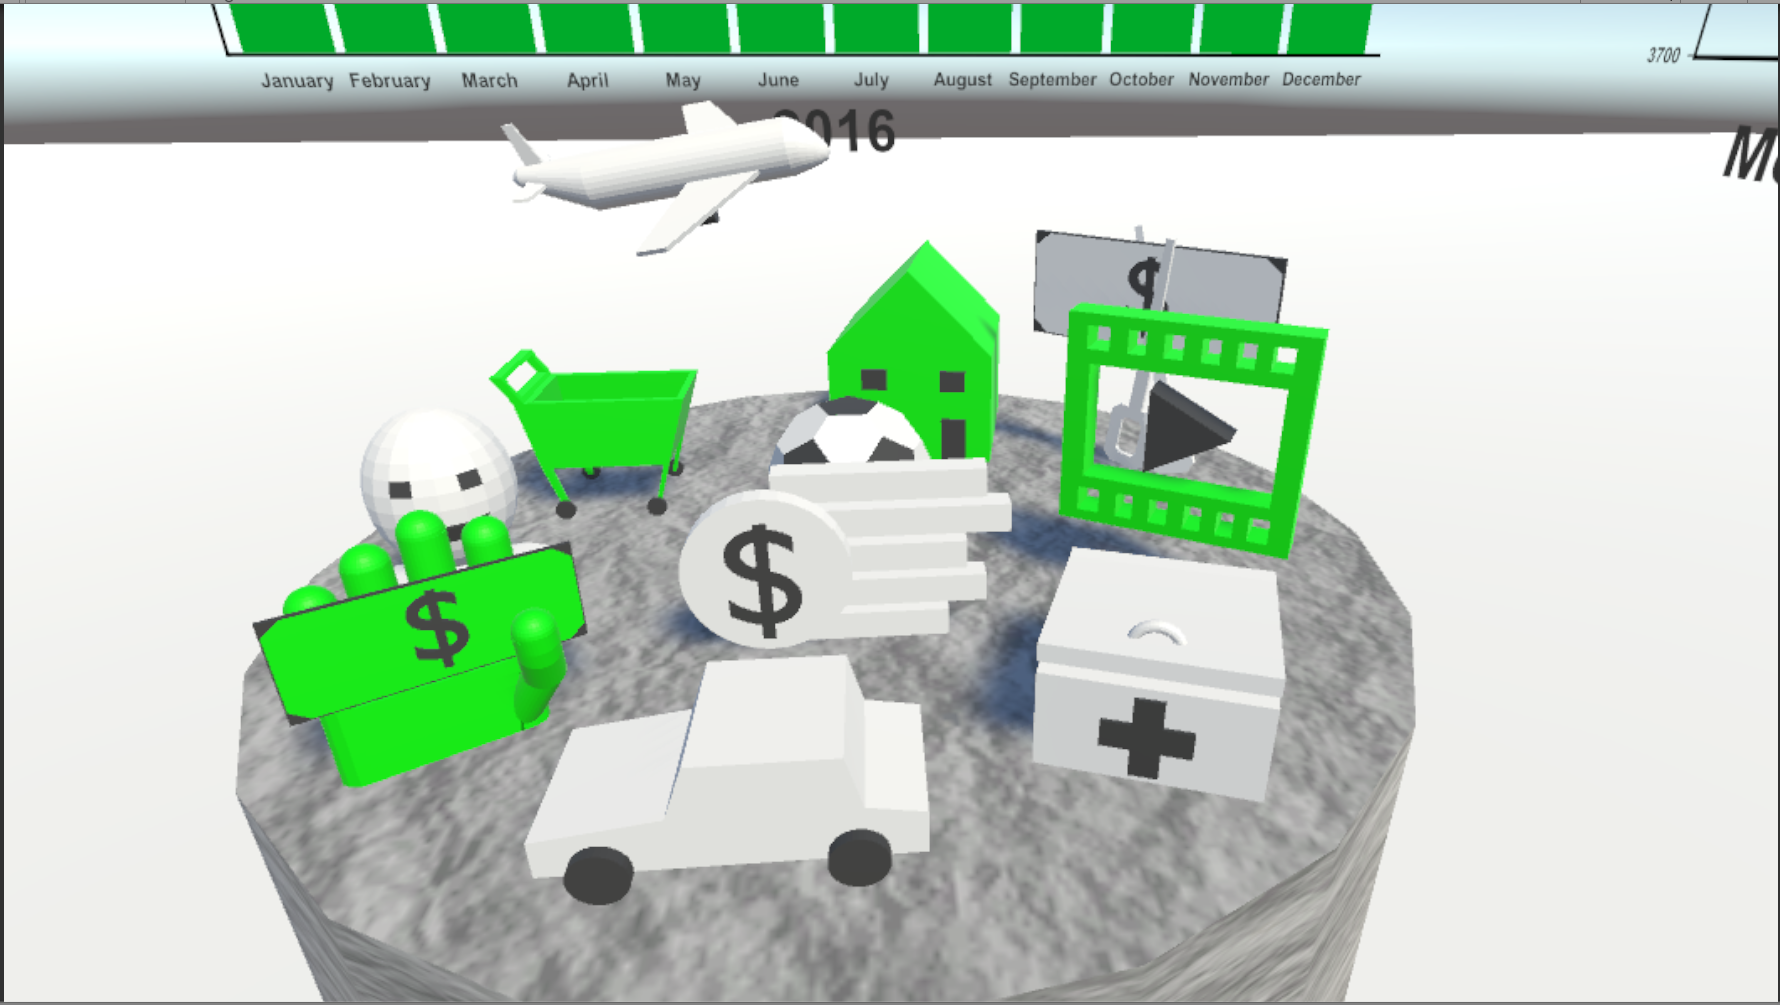
\includegraphics[width=2.8cm]{03_Figures/08_Development/View4_CategoriesFiltering.png}
		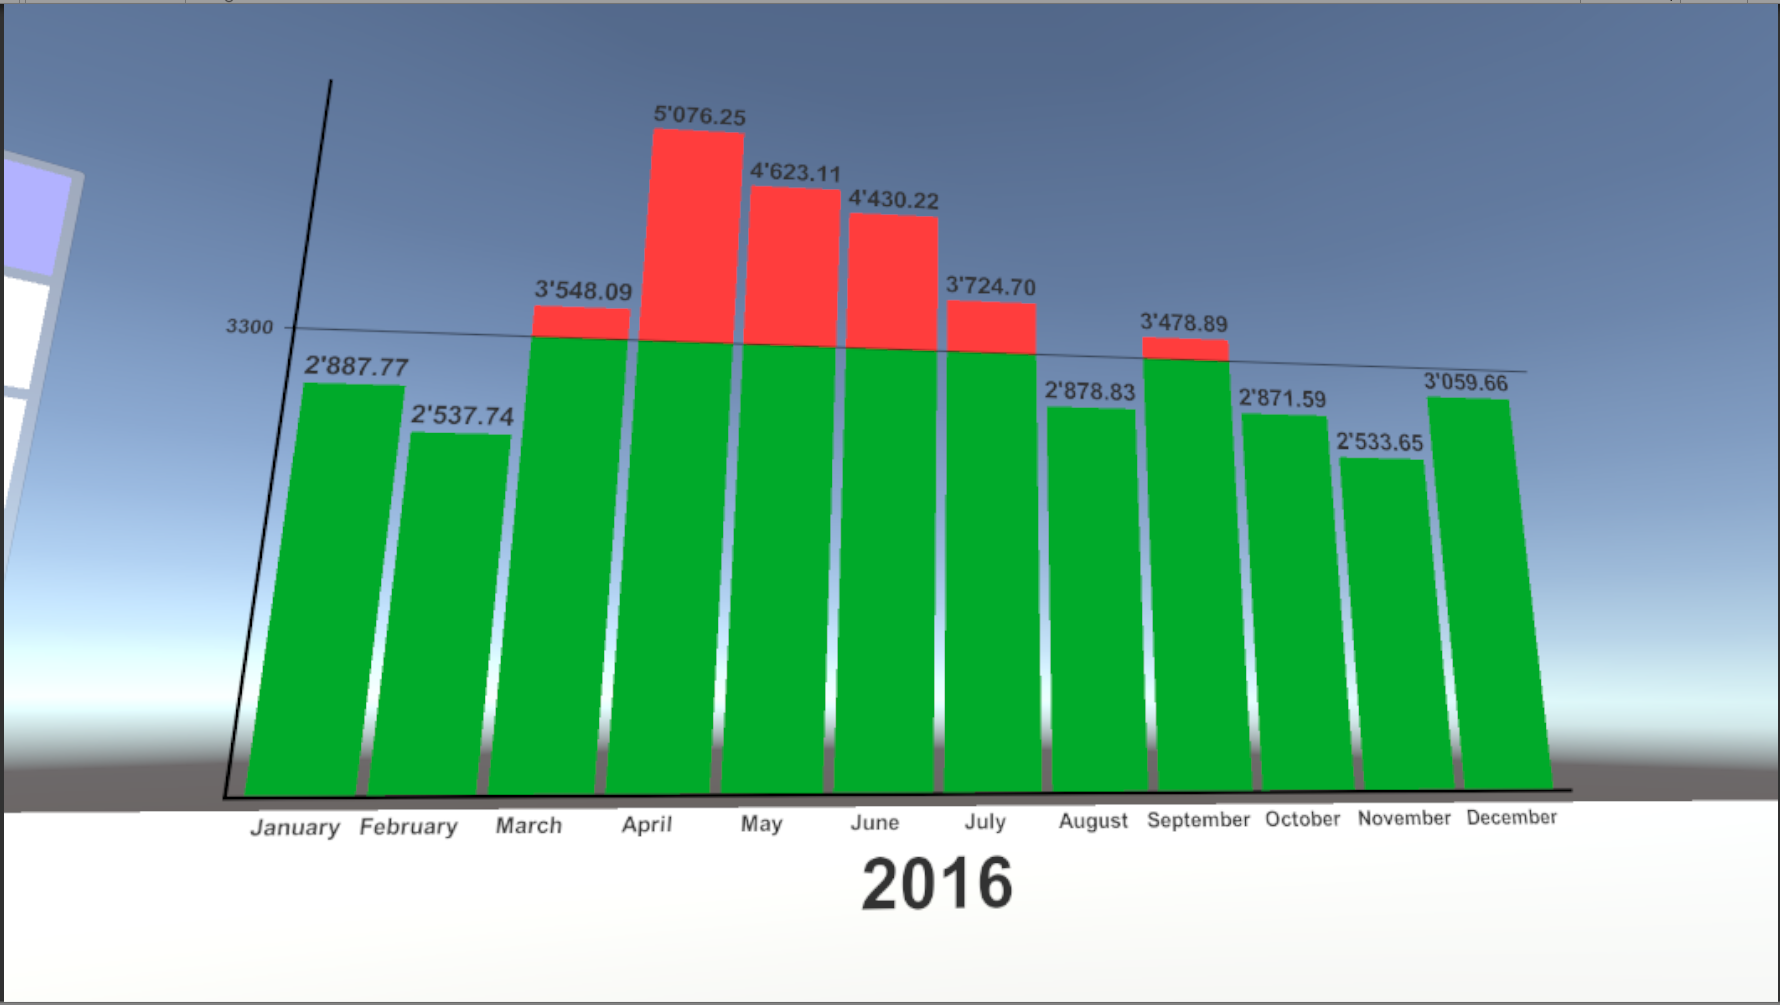
\includegraphics[width=2.8cm]{03_Figures/08_Development/View1_YearOverview.png}
		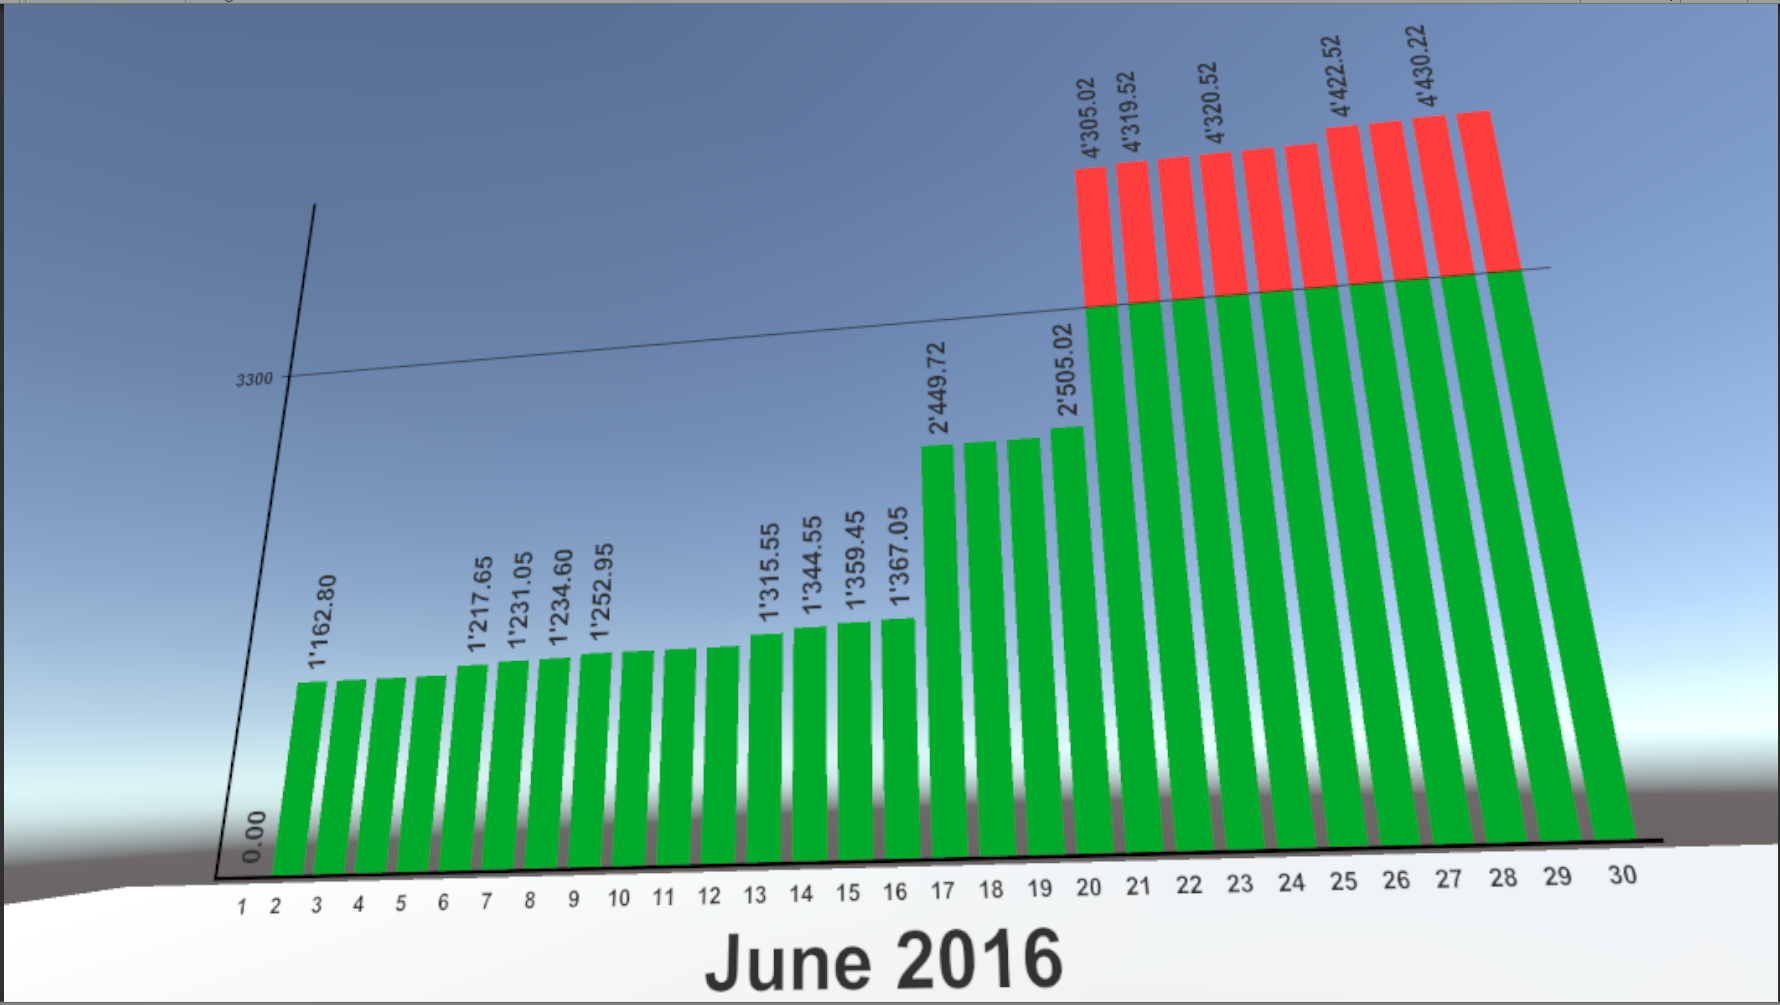
\includegraphics[width=2.8cm]{03_Figures/08_Development/View2_MonthOverview.png}
		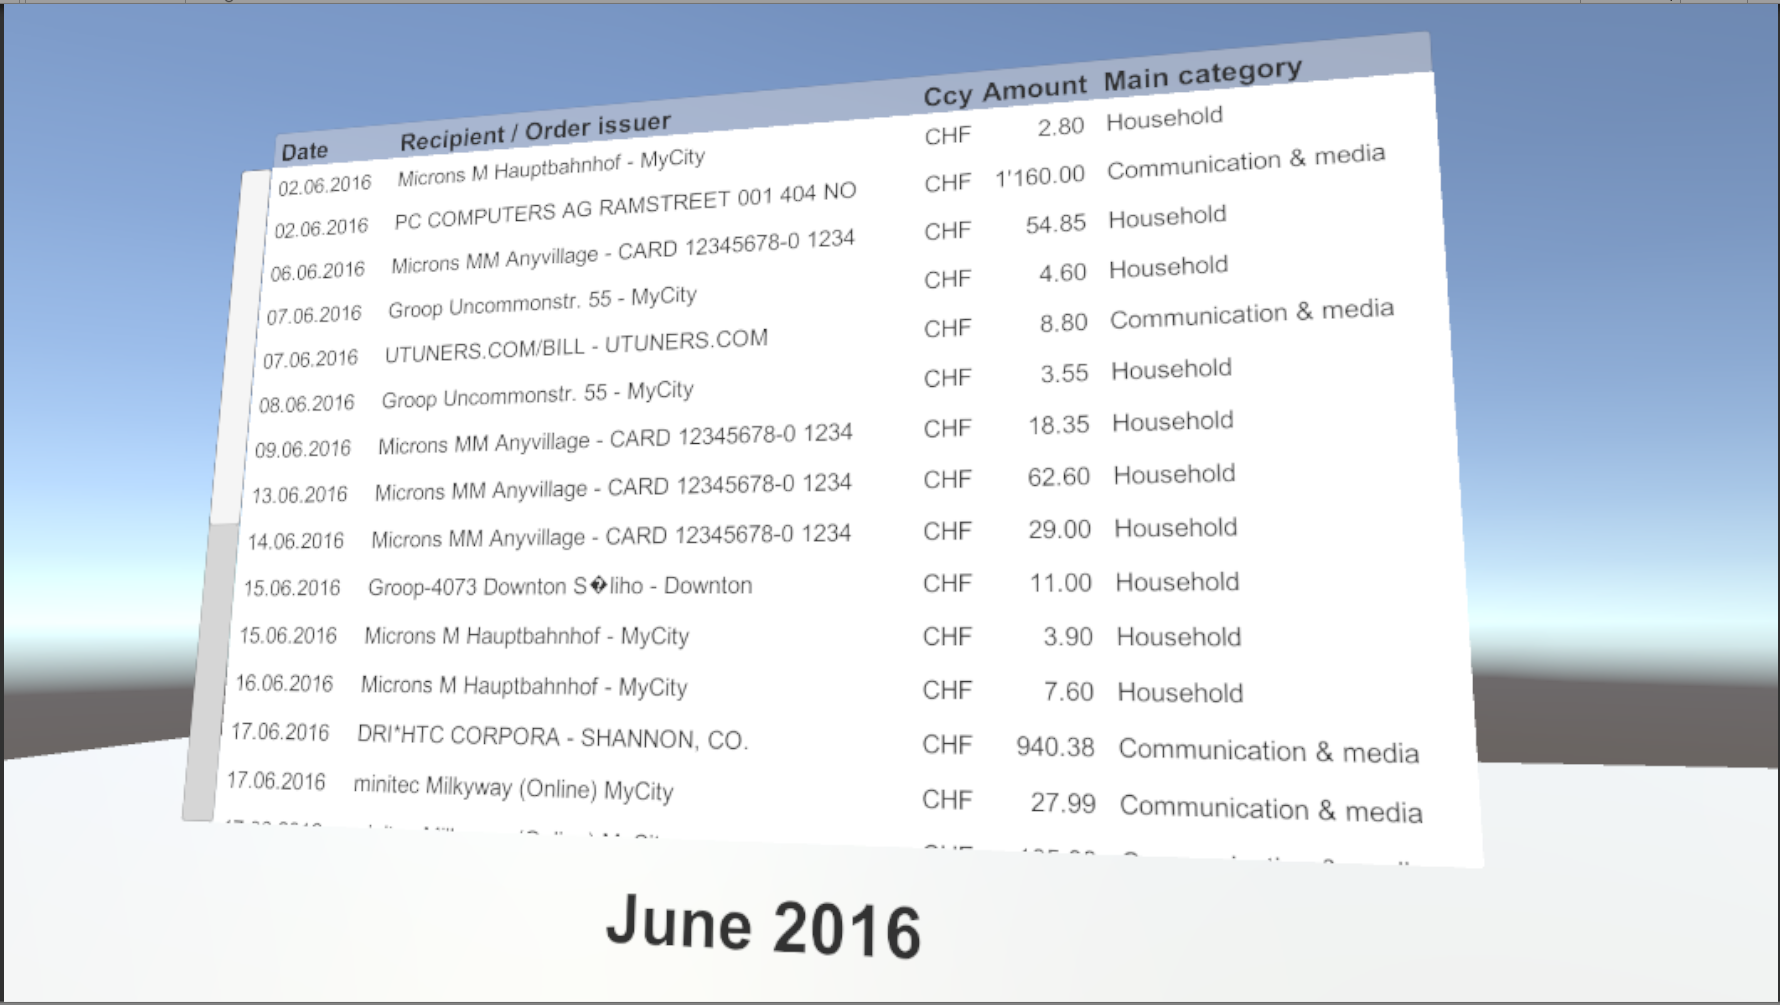
\includegraphics[width=2.8cm]{03_Figures/08_Development/View5_FinTransactionsOverview.png}
		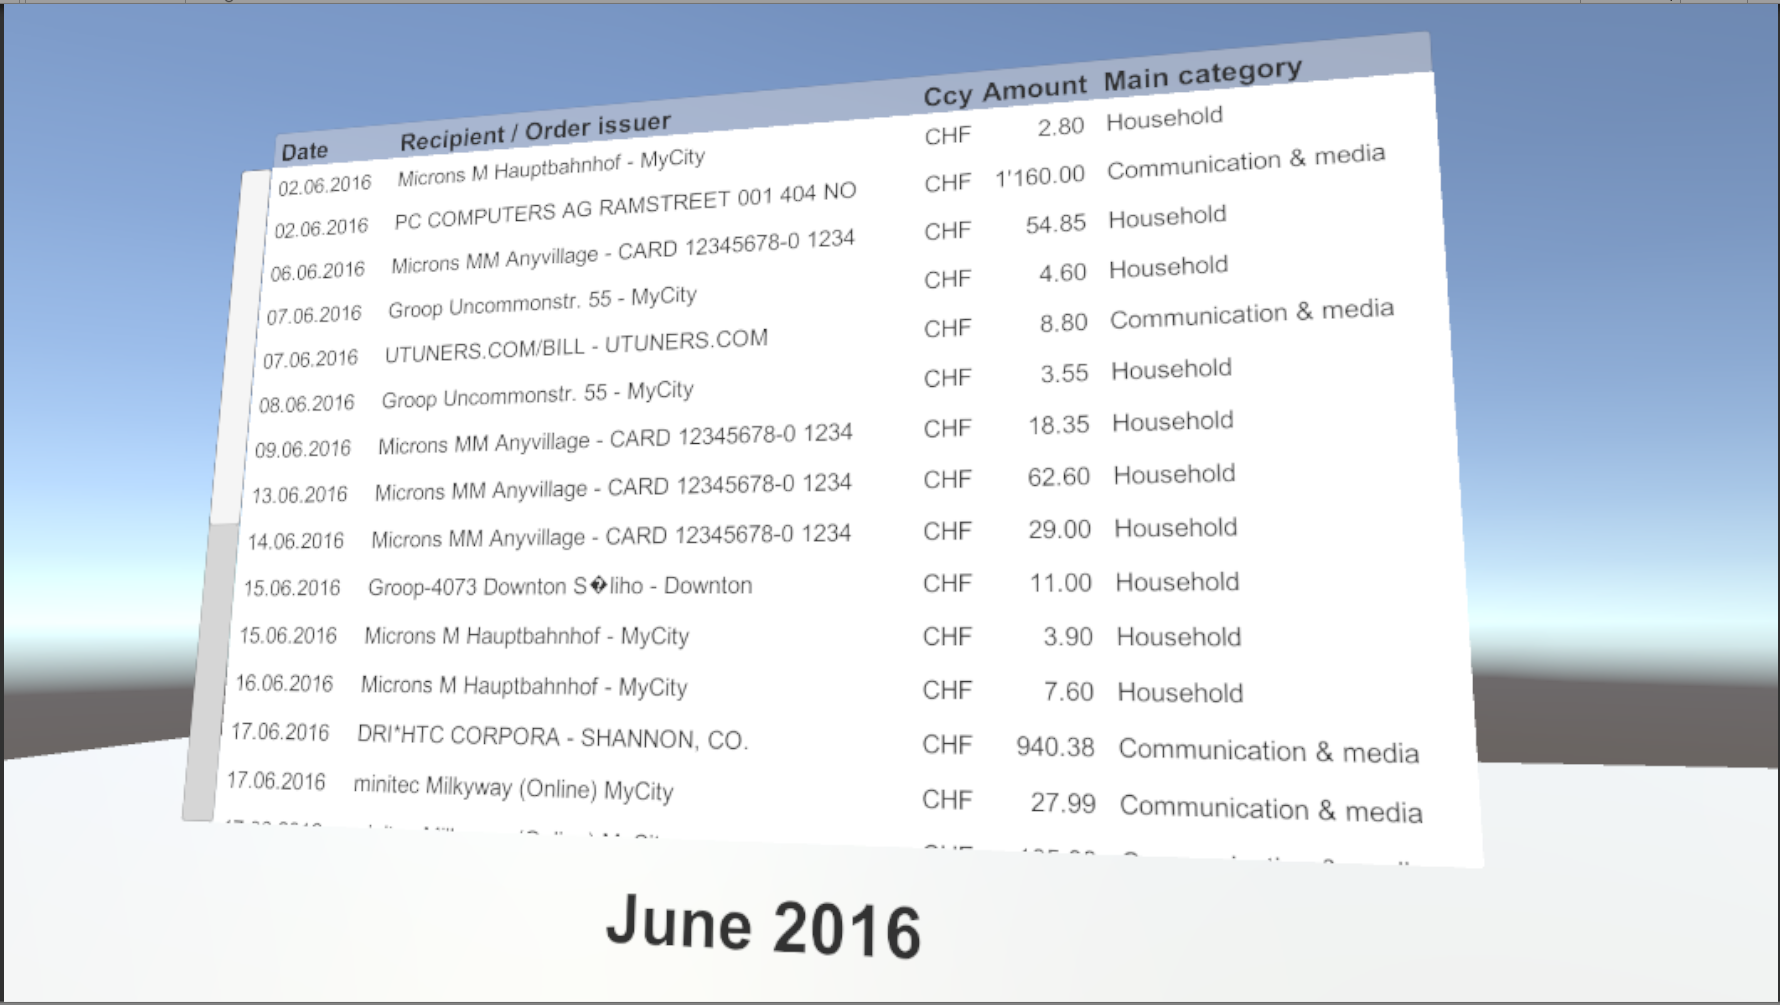
\includegraphics[width=2.8cm]{03_Figures/08_Development/View5_FinTransactionsOverview.png}
		\caption{Visualised flow of views in prototype for Scenario 1}
		\label{fig:scenariooneprototype}
	\end{center}
\end{figure}


\textbf{Evaluation:} Depending on the amount of rows in the table, the exclusivity can be rated a bit higher or not. Selecting a specific day in the Month Overview clearly helps to reduce the amount of rows, but might require additional interaction steps if it is not known on what exact date the transaction was executed. Since it is not directly possible to search for a specific booking text or similar, some interpretation on the table rows is required.
\begin{itemize}[noitemsep,nolistsep]
	\item Min. number of steps: \textbf{3 - 5}
	\item Exclusivity: \textbf{Medium} (with filtered day), \textbf{Low} (without)
	\item Comprehensibility: \textbf{Medium}
\end{itemize}


%-----------------------------------
%	SUBSUBSECTION 1
%-----------------------------------

\subsubsection{Conclusion}

tbd Table \ref{tbl:scenarioonecomparison}

\begin{table}[t]
	\begin{center}
		\begin{tabular}{ | p{3.5cm} | p{3cm} | p{3cm} | p{3cm} | } 
			\hline
			\textbf{Metric} & \textbf{E-banking} & \textbf{Prototype} & \textbf{Verdict} \\
			\hline
				Min. no. of steps: &  & 3 - 5 &  \\
			\hline
				Exclusivity: &  & Medium / Low &  \\
			\hline
				Comprehensibility: &  & Medium &  \\
			\hline
		\end{tabular}
		\caption{Scenario 1: Comparison of prototype and e-banking}
		\label{tbl:scenarioonecomparison}
	\end{center}
\end{table}


%-----------------------------------
%	SUBSECTION 2
%-----------------------------------

\subsection{Scenario 2}

\textbf{Scenario title:} \scentwo

\textbf{Exemplary situation:} Since their first child was born, a family is wondering how their household and travelling expenses have changed compared to previous years.



%-----------------------------------
%	SUBSUBSECTION 1
%-----------------------------------

\subsubsection{UBS e-Banking}

tbd

\textbf{Evaluation:} 
\begin{itemize}[noitemsep,nolistsep]
	\item Min. number of steps: \textbf{}
	\item Exclusivity: \textbf{}
	\item Comprehensibility: \textbf{}
\end{itemize}


%-----------------------------------
%	SUBSUBSECTION 2
%-----------------------------------

\subsubsection{Prototype Application}

With the prototype application, the answer to this scenario can again be found in 3-5 interaction steps, depending on whether more detailed information from a single month is also looked at. The visualised flow for this scenario is shown in Figure \ref{fig:scenariotwoprototype}.
\begin{enumerate}[noitemsep,nolistsep]
	\item Activate "Household" category (View 4)
	\item Activate "Vacation \& travel" category (View 4)
	\item OPTIONAL: Click on a month in the Year Overview bar chart (View 1)
	\item Click on the previous year in the Year Selection (View 3)
	\item OPTIONAL: Click on a month in the Year Overview bar chart (View 1)
\end{enumerate}
\begin{figure}[h]
	\begin{center}
		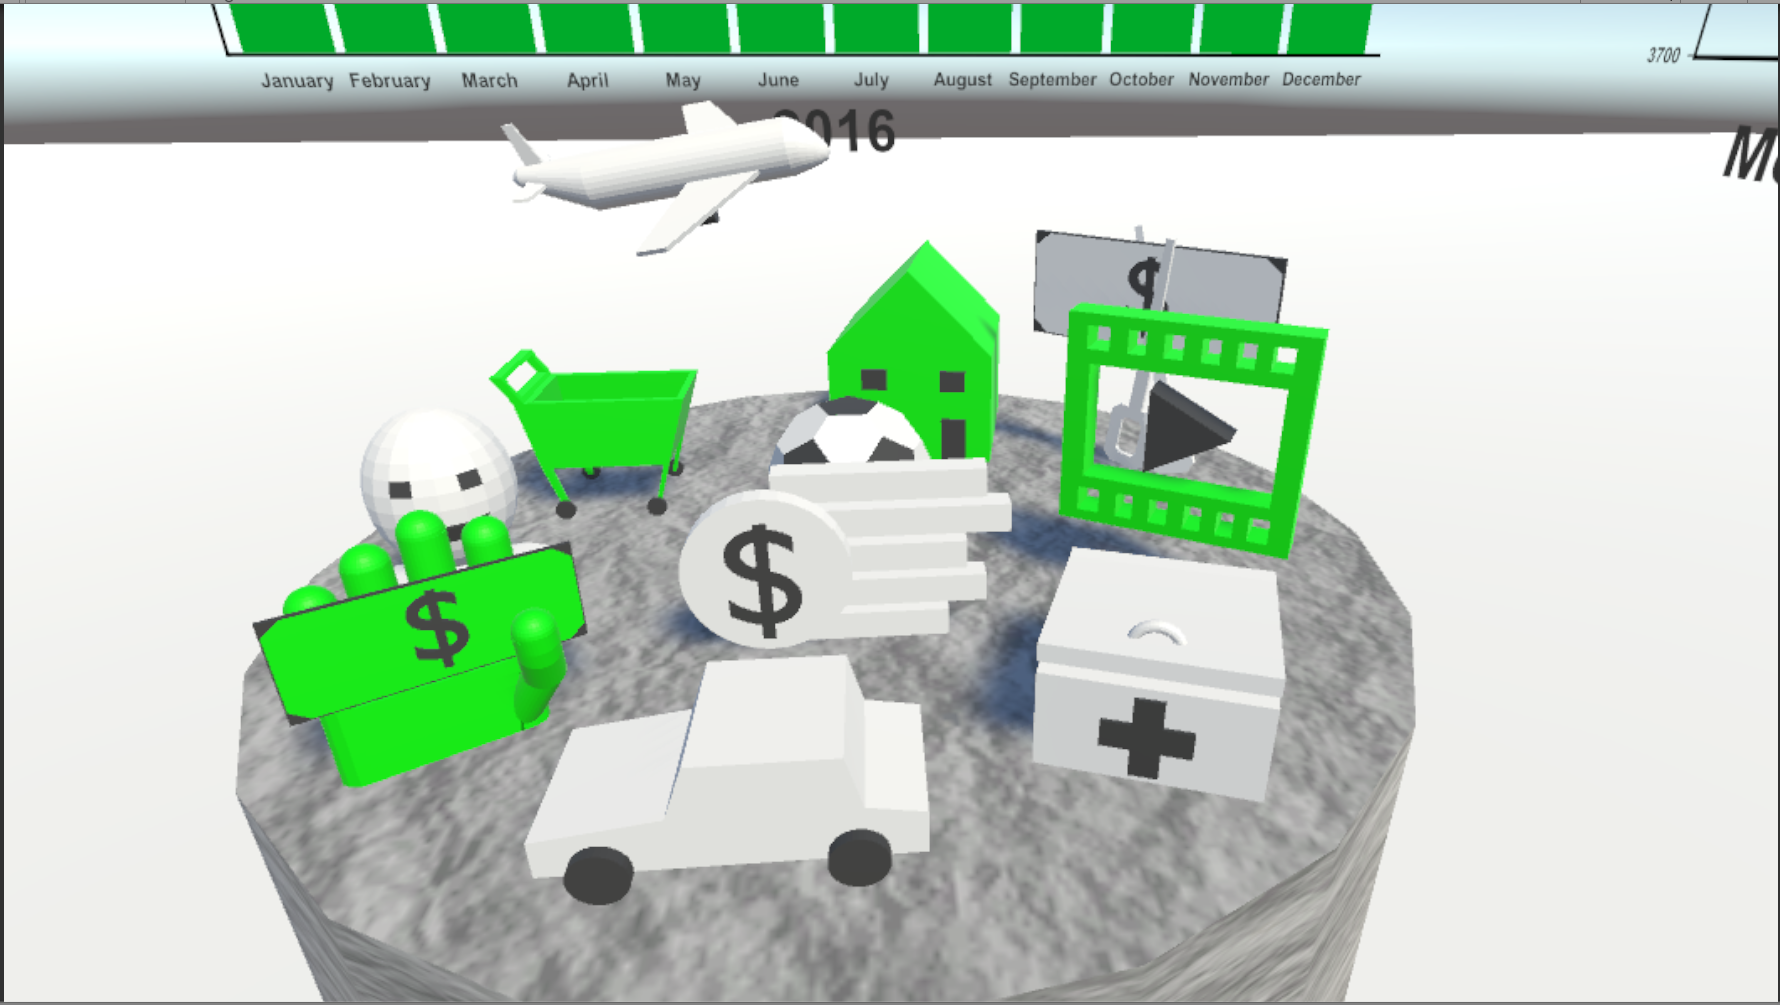
\includegraphics[width=2.8cm]{03_Figures/08_Development/View4_CategoriesFiltering.png}
		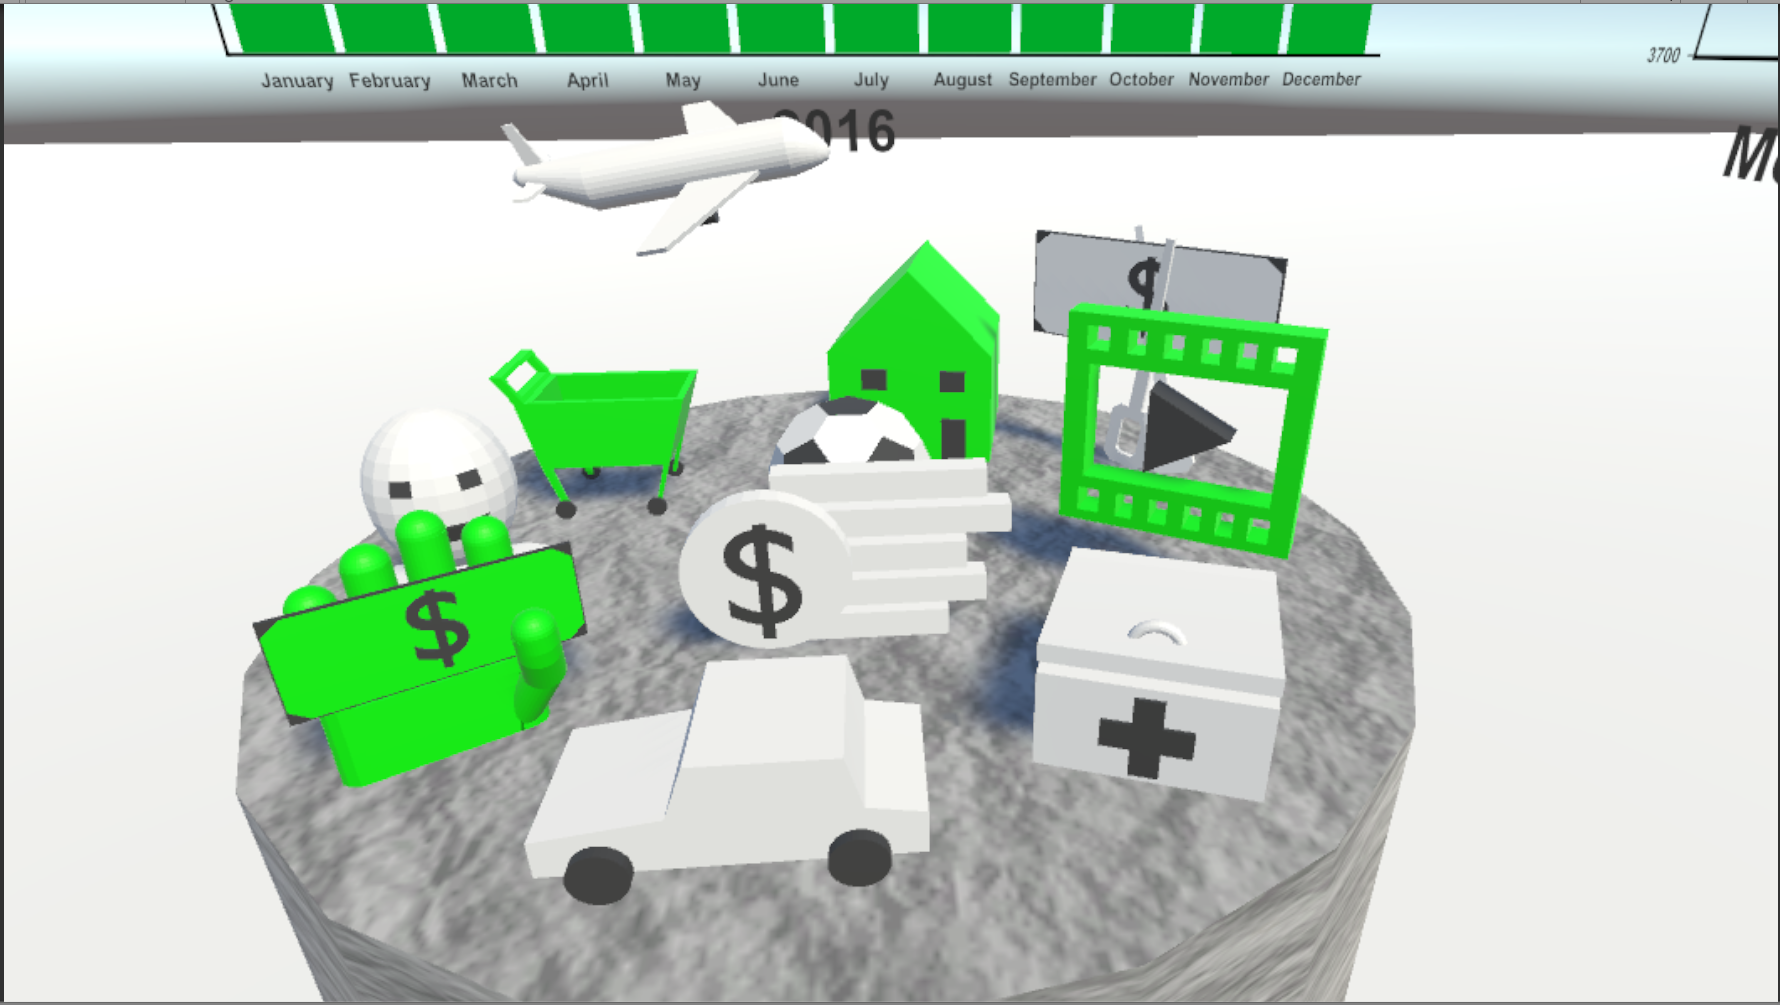
\includegraphics[width=2.8cm]{03_Figures/08_Development/View4_CategoriesFiltering.png}
		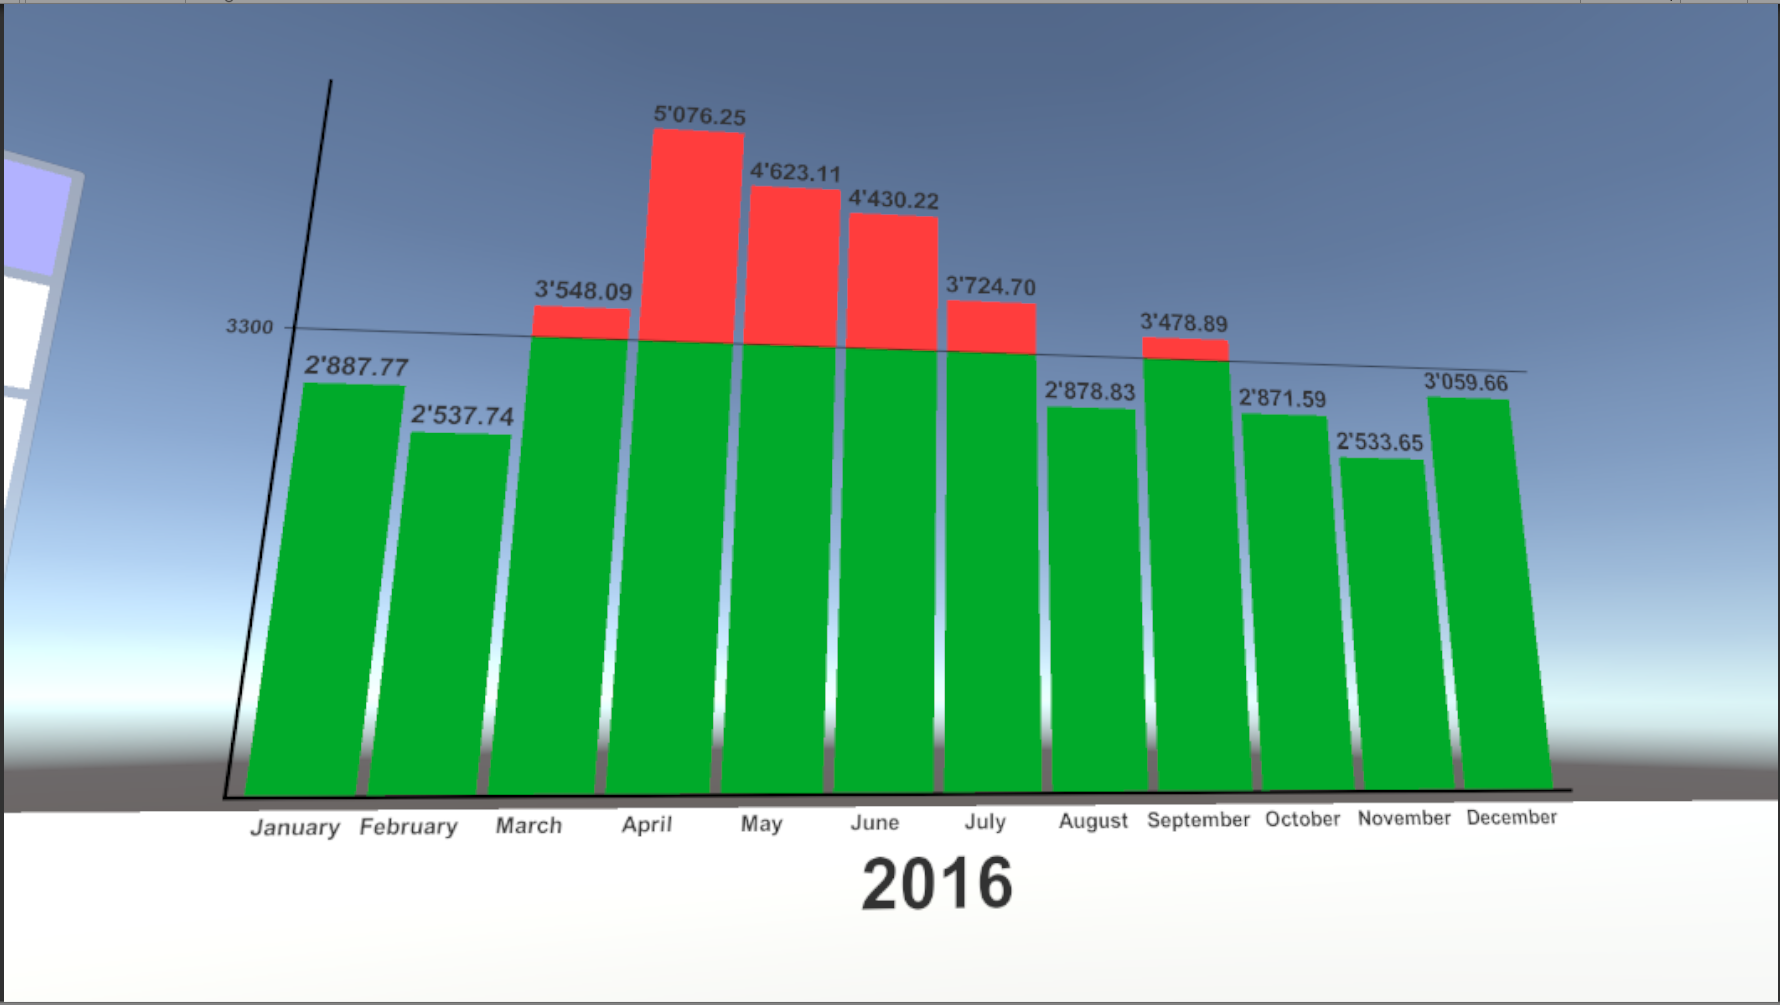
\includegraphics[width=2.8cm]{03_Figures/08_Development/View1_YearOverview.png}
		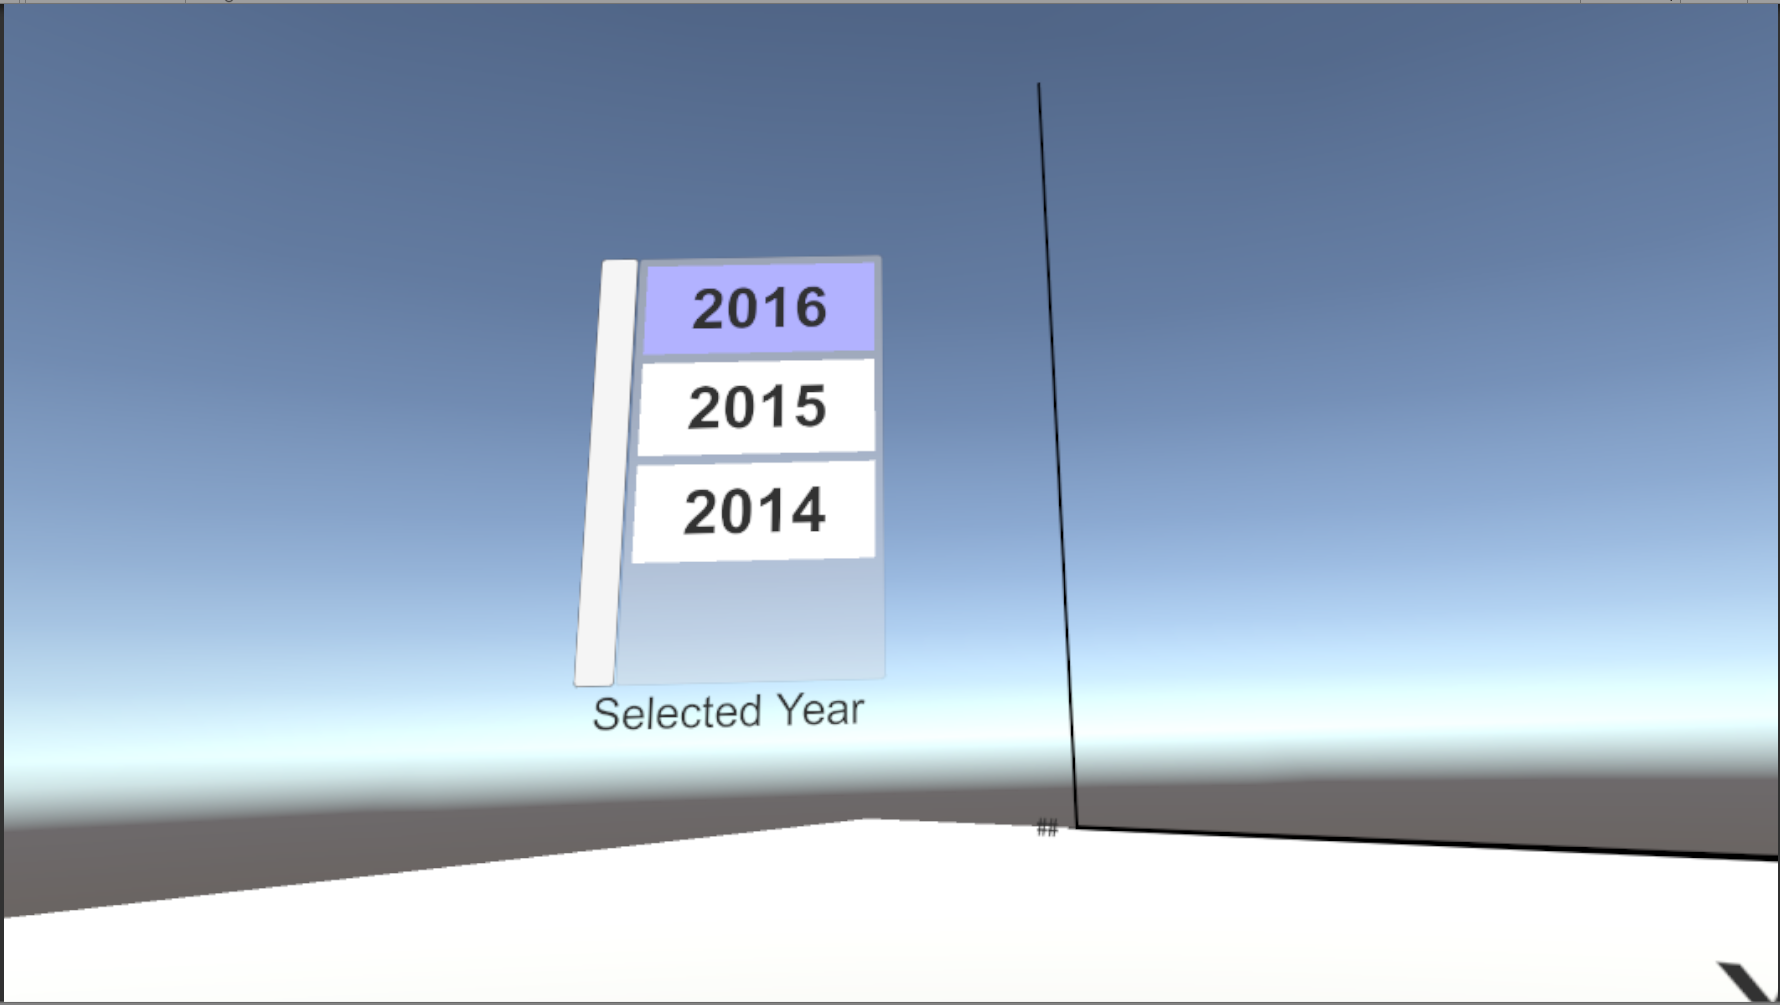
\includegraphics[width=2.8cm]{03_Figures/08_Development/View3_YearSelection.png}
		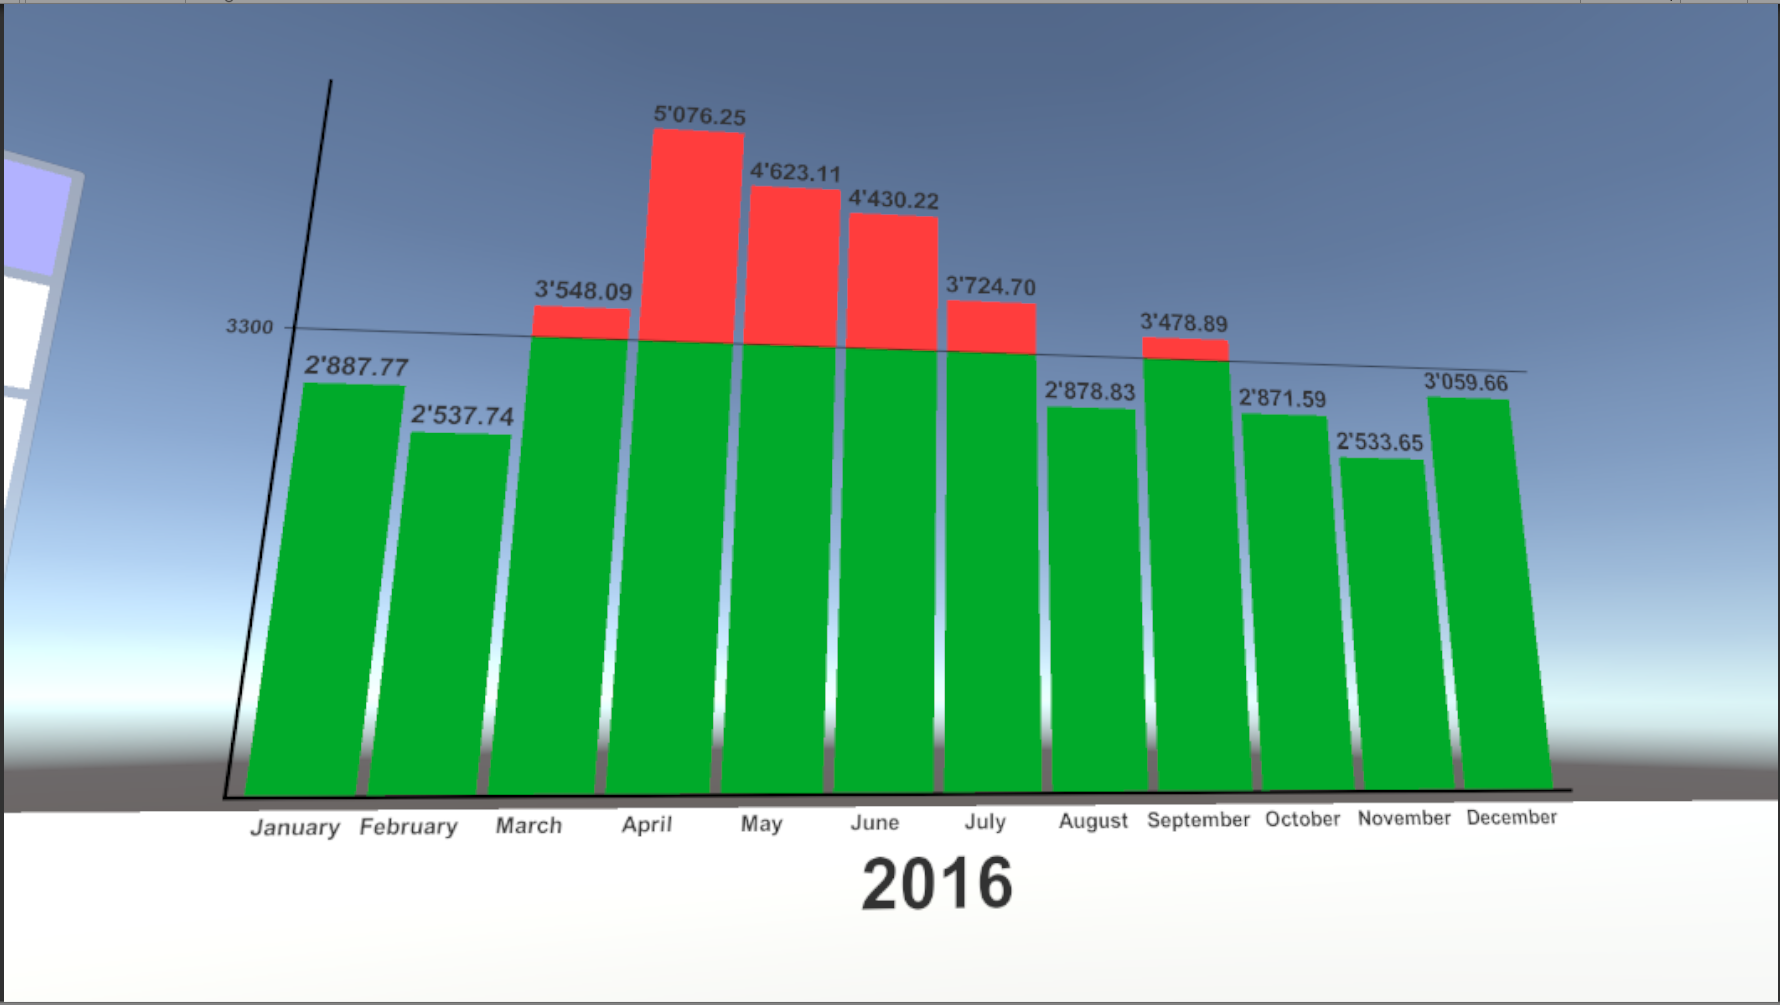
\includegraphics[width=2.8cm]{03_Figures/08_Development/View1_YearOverview.png}
		\caption{Visualised flow of views in prototype for Scenario 2}
		\label{fig:scenariotwoeprototype}
	\end{center}
\end{figure}

\textbf{Evaluation:} Since the focus is on comparing the expenses for two categories over the whole course of a year, the exclusivity is high in this case with the multiple categories that can be filtered for. Also when selecting an individual month, it only shows the data of the activated categories. As for the comprehensibility, since it is not possible to have both years next to each other, switching in between them is necessary and thus requires some interpretation. Once the data has been cached, the switching between years however becomes very fast to execute.
\begin{itemize}[noitemsep,nolistsep]
	\item Min. number of steps: \textbf{3 - 5}
	\item Exclusivity: \textbf{High}
	\item Comprehensibility: \textbf{Medium}
\end{itemize}


%-----------------------------------
%	SUBSUBSECTION 1
%-----------------------------------

\subsubsection{Conclusion}

tbd Table \ref{tbl:scenariotwocomparison}

\begin{table}[t]
	\begin{center}
		\begin{tabular}{ | p{3.5cm} | p{3cm} | p{3cm} | p{3cm} | } 
			\hline
			\textbf{Metric} & \textbf{E-banking} & \textbf{Prototype} & \textbf{Verdict} \\
			\hline
			Min. no. of steps: &  & 3 - 5 &  \\
			\hline
			Exclusivity: &  & High &  \\
			\hline
			Comprehensibility: &  & Medium &  \\
			\hline
		\end{tabular}
		\caption{Scenario 2: Comparison of prototype and e-banking}
		\label{tbl:scenariotwocomparison}
	\end{center}
\end{table}


%-----------------------------------
%	SUBSECTION 3
%-----------------------------------

\subsection{Scenario 3}

\textbf{Scenario title:} \scenthree

\textbf{Exemplary situation:} Noticing that his account balance is down to zero a week before the next salary payment is expected, a user is wondering what expense(s) lead to this unexpected situation.


%-----------------------------------
%	SUBSUBSECTION 1
%-----------------------------------

\subsubsection{UBS e-Banking}

tbd

\textbf{Evaluation:} 
\begin{itemize}[noitemsep,nolistsep]
	\item Min. number of steps: \textbf{}
	\item Exclusivity: \textbf{}
	\item Comprehensibility: \textbf{}
\end{itemize}


%-----------------------------------
%	SUBSUBSECTION 2
%-----------------------------------

\subsubsection{Prototype Application}

The answer to this scenario can be found with only 2-5 interaction steps in the prototype application, depending how spread out the suspicious payments were over the selected month. The visualised flow for this scenario is shown in Figure \ref{fig:scenariothreeprototype}.
\begin{enumerate}[noitemsep,nolistsep]
	\item Toggle-activate all categories (View 4)
	\item Click on the current month in the Year Overview bar chart (View 1)
	\item OPTIONAL: Click on a day with a big jump in expenses in the Month Overview bar chart (View 2)
	\item OPTIONAL: Scroll down the list of transactions if there are too many (View 5)
	\item OPTIONAL: Click on the suspicious transaction in the List of Transactions (View 5)
\end{enumerate}
\begin{figure}[h]
	\begin{center}
		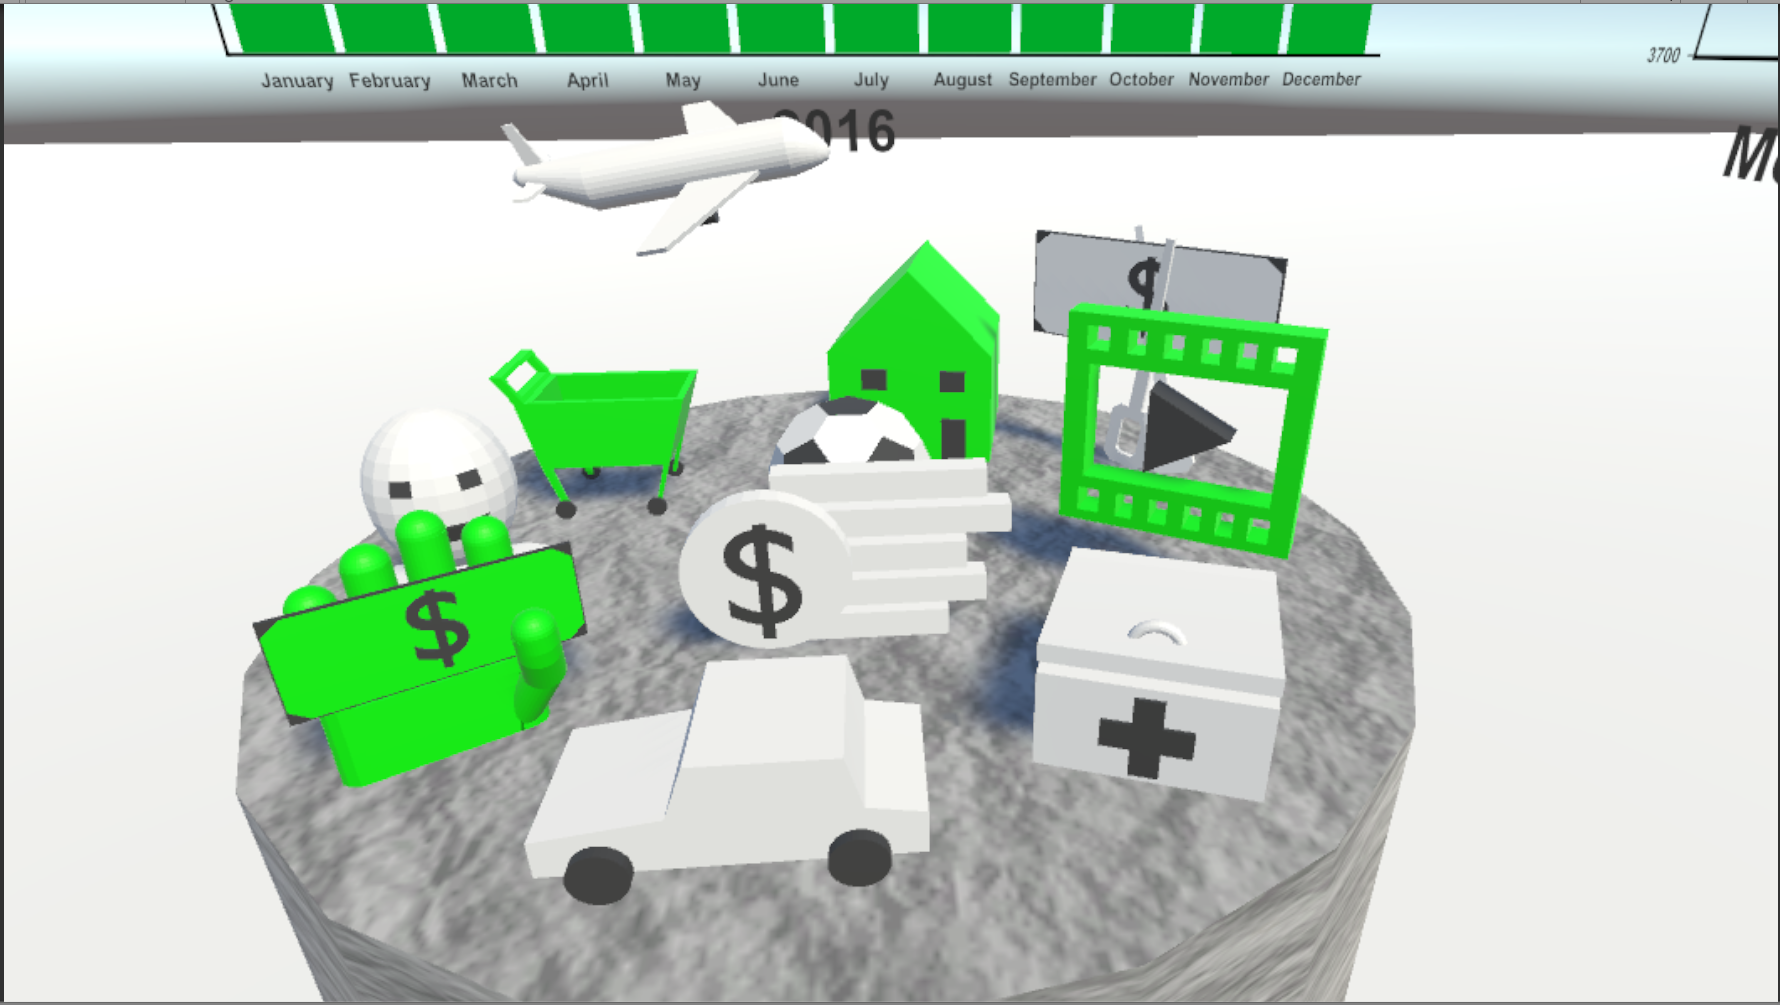
\includegraphics[width=2.8cm]{03_Figures/08_Development/View4_CategoriesFiltering.png}
		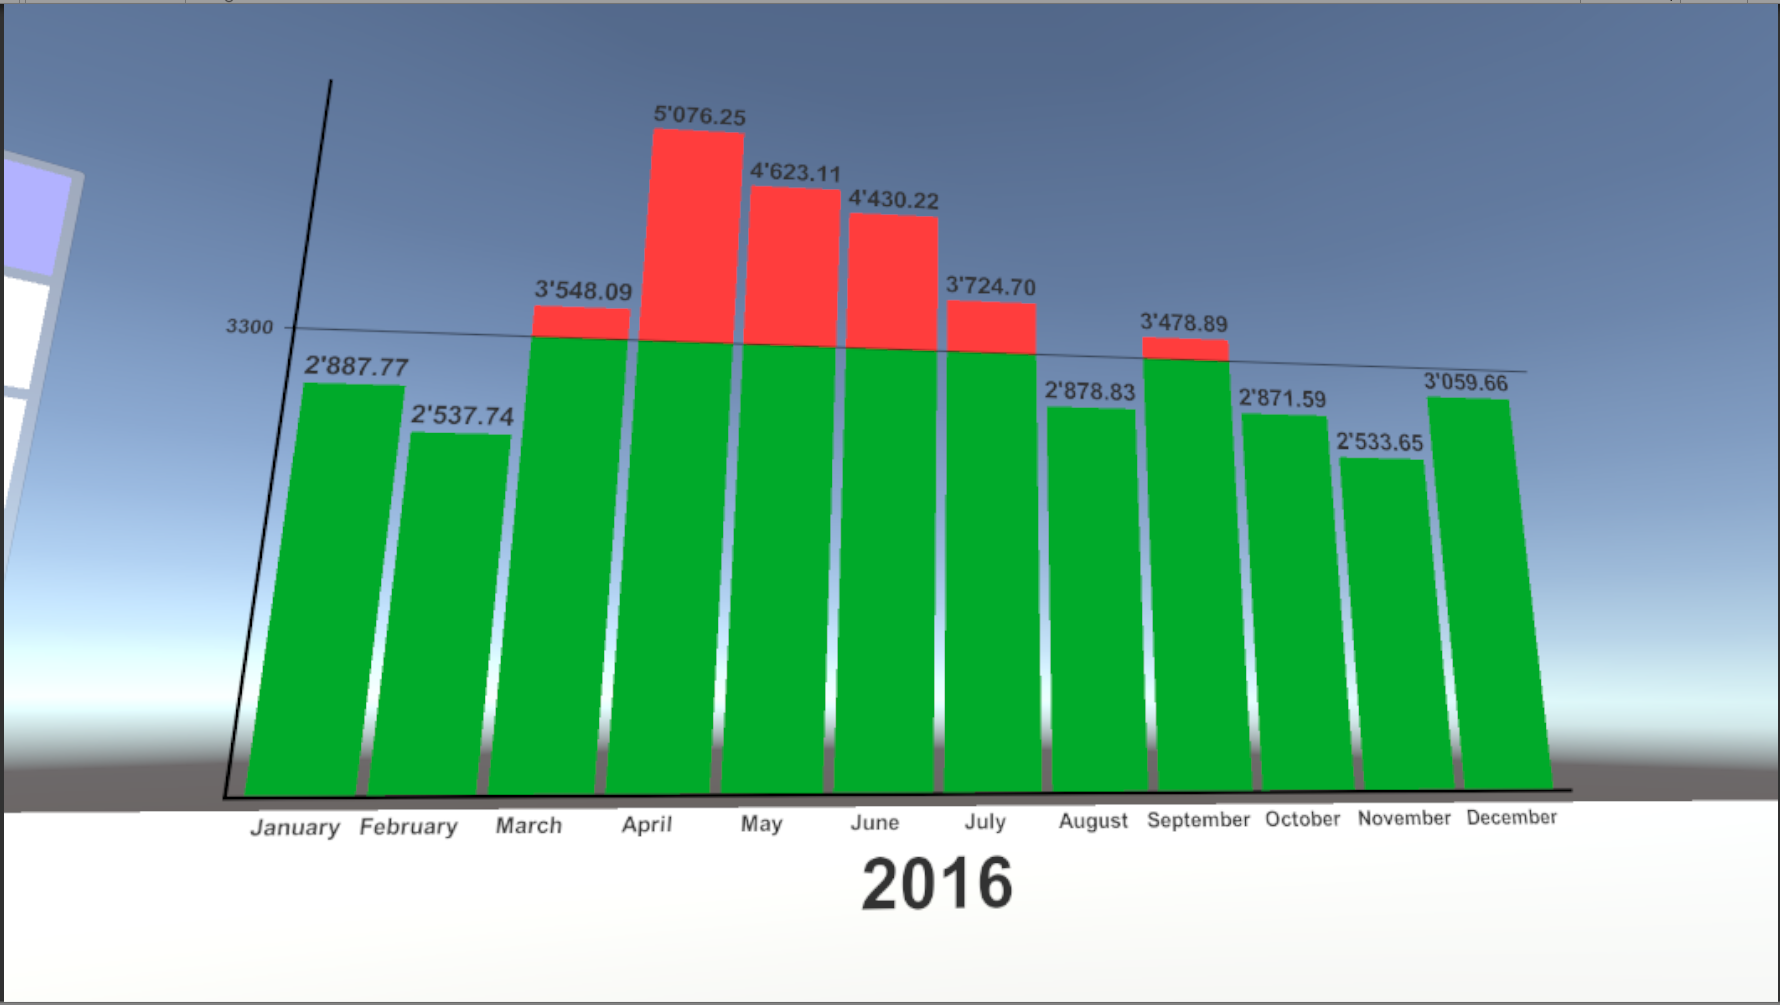
\includegraphics[width=2.8cm]{03_Figures/08_Development/View1_YearOverview.png}
		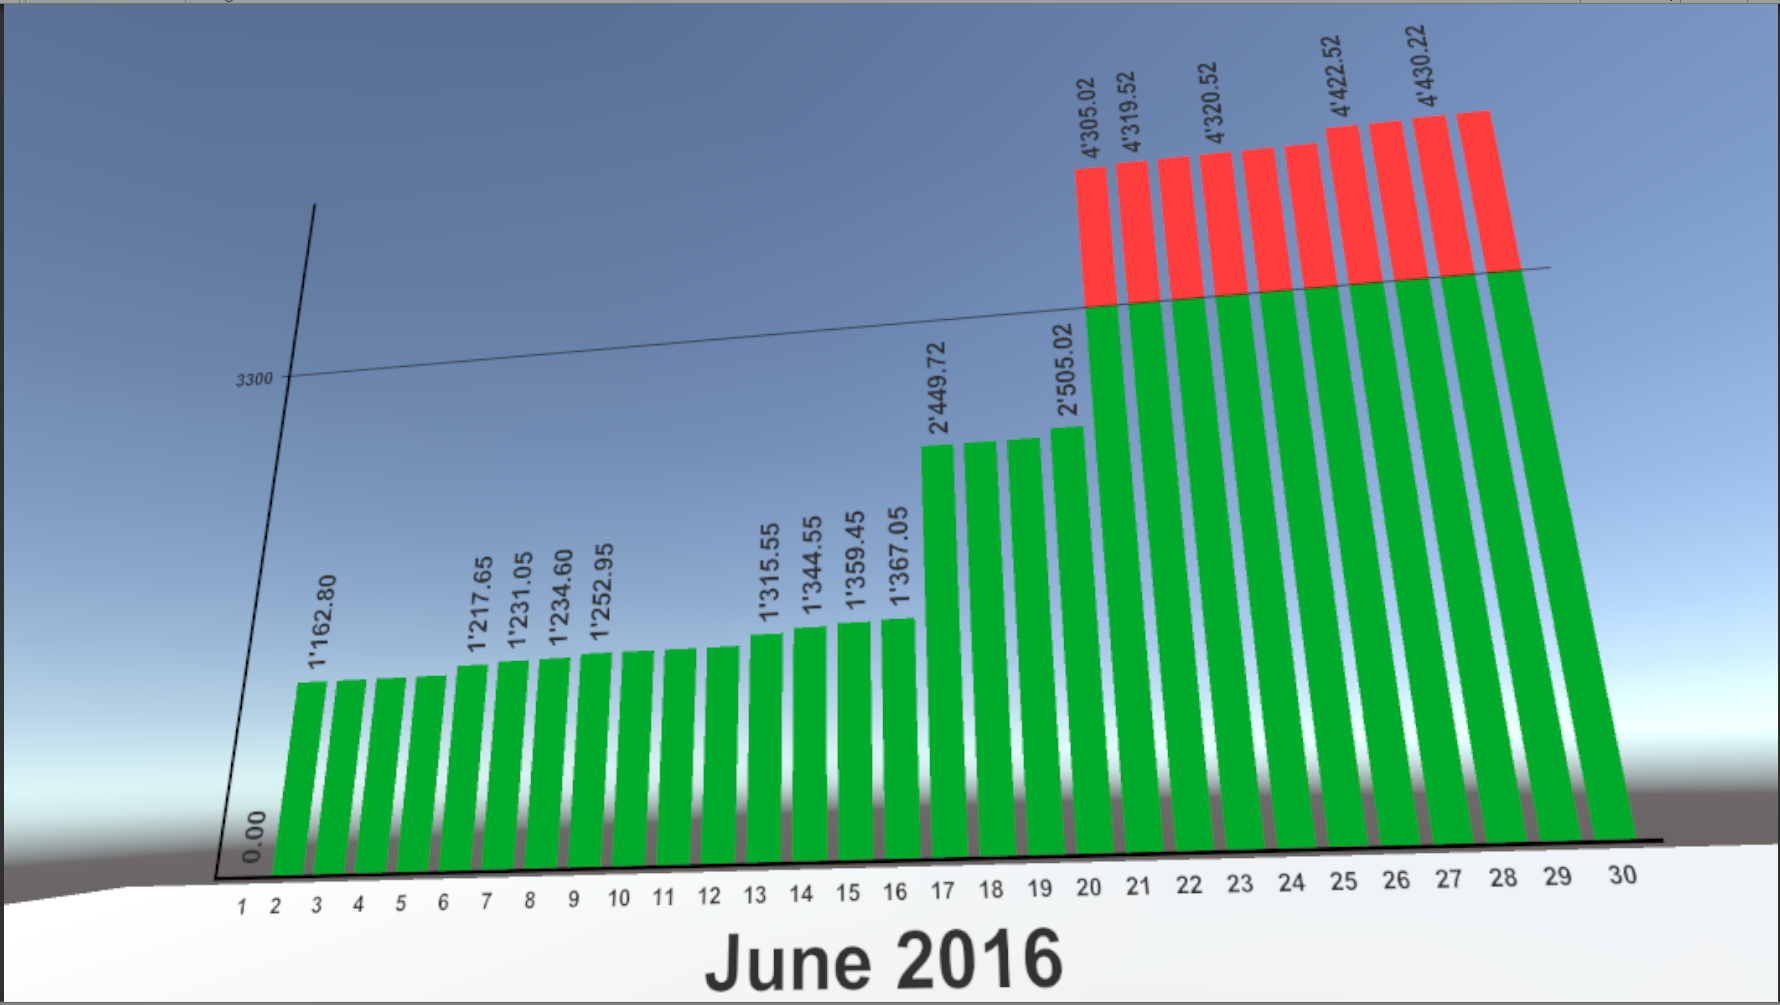
\includegraphics[width=2.8cm]{03_Figures/08_Development/View2_MonthOverview.png}
		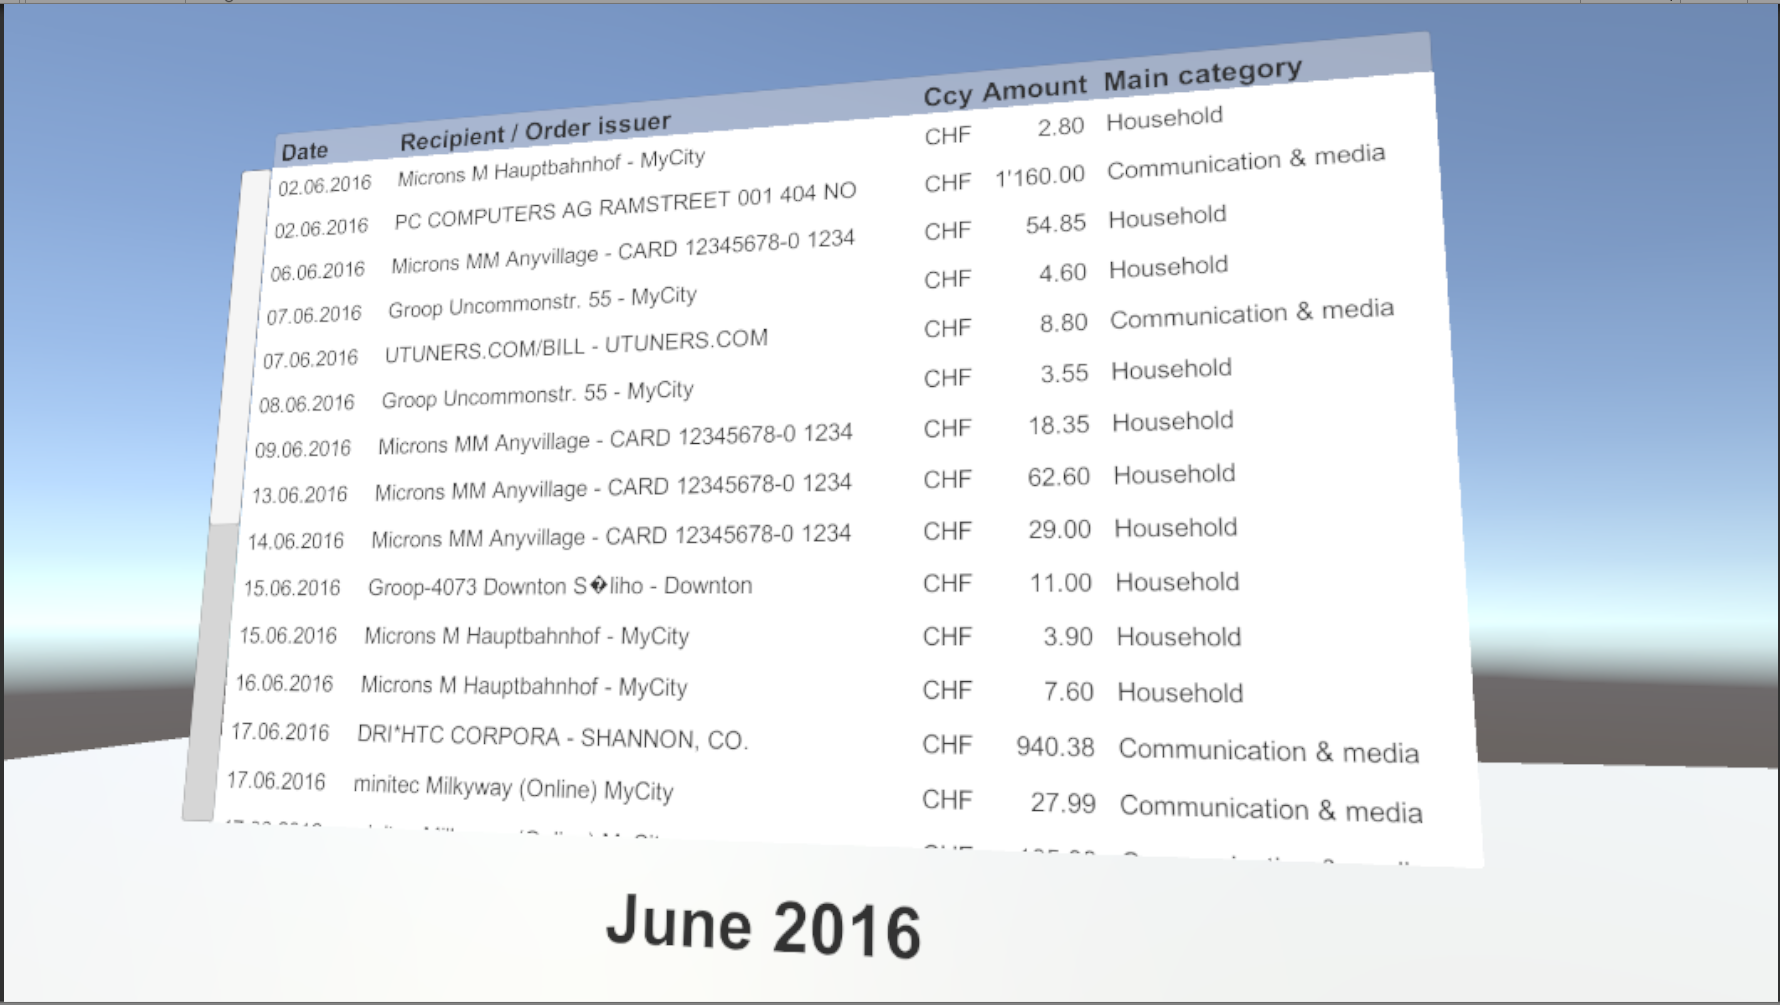
\includegraphics[width=2.8cm]{03_Figures/08_Development/View5_FinTransactionsOverview.png}
		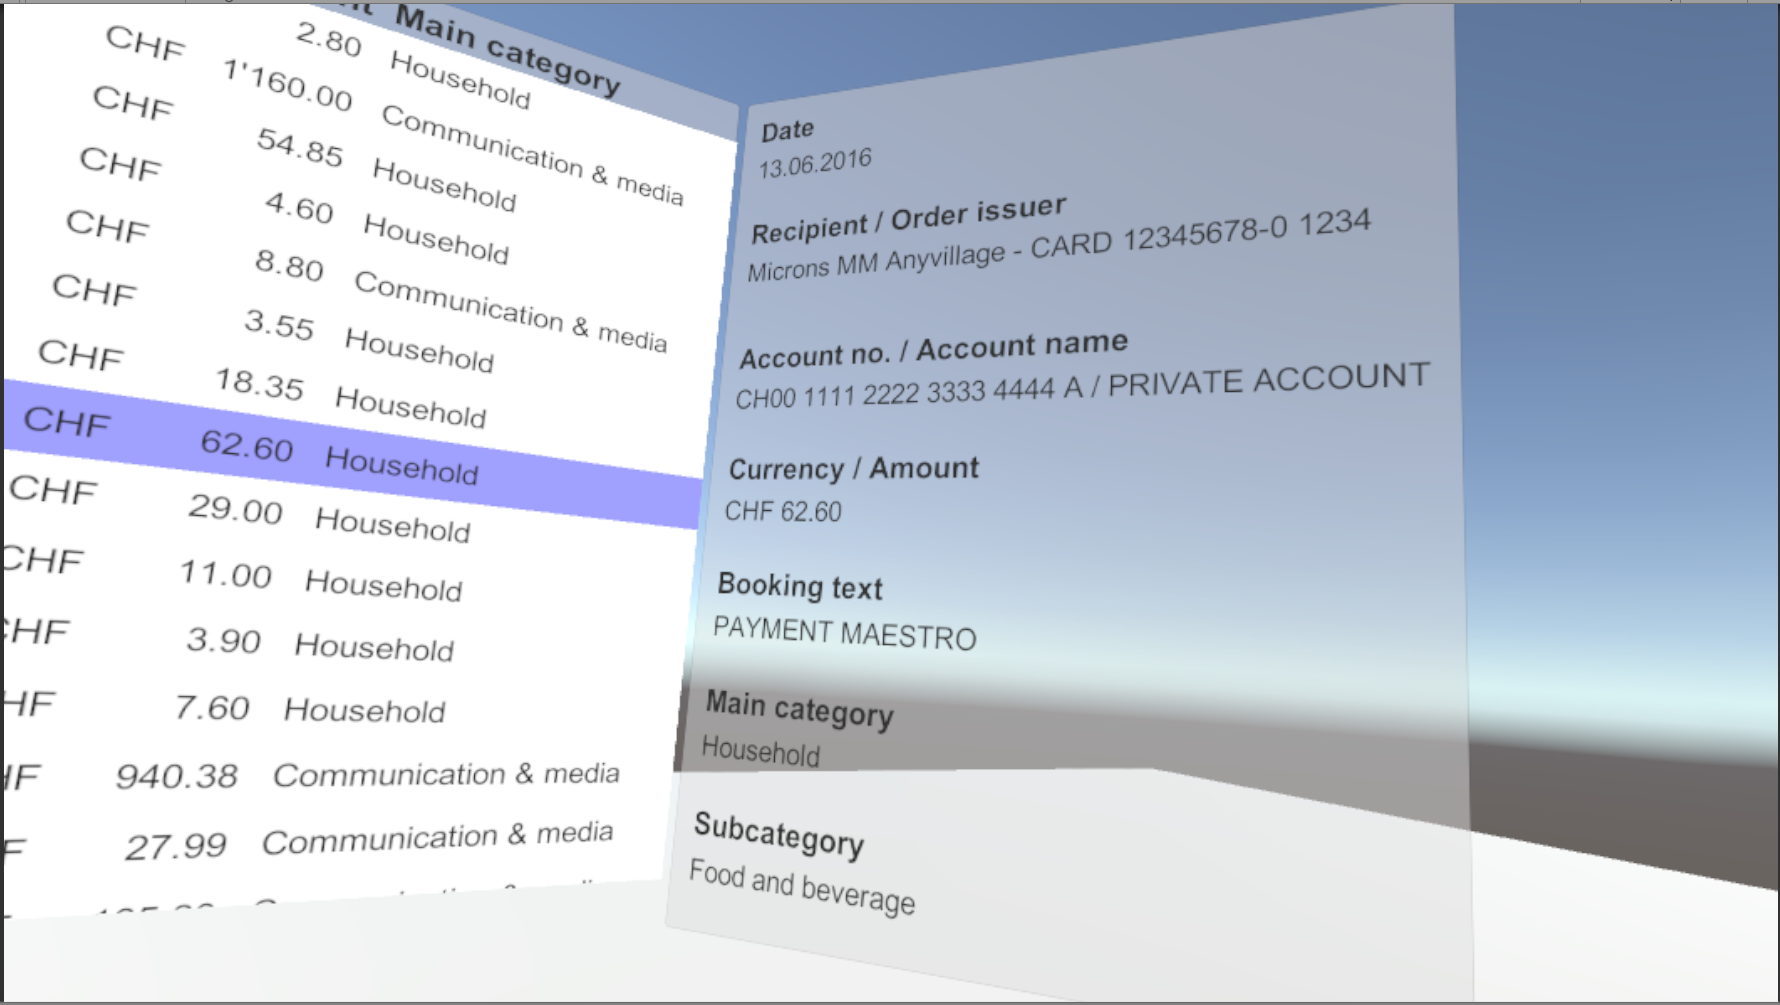
\includegraphics[width=2.8cm]{03_Figures/08_Development/View6_FinTransactionDetails.png}
		\caption{Visualised flow of views in prototype for Scenario 3}
		\label{fig:scenariothreeprototype}
	\end{center}
\end{figure}

\textbf{Evaluation:} When all categories are activated, the Month Overview should give a clear indication on which day(s) unexpected high transactions were executed. If it focuses on a single day, it can be selected and then the table shows only this very specific transactions, leading to a medium exclusivity. If it is however more spread out over the whole month, the exclusivity is rather low. From a comprehensibility aspect, the user is still required to go through the list and and find the suspicious transactions by himself.
\begin{itemize}[noitemsep,nolistsep]
	\item Min. number of steps: \textbf{2 - 5}
	\item Exclusivity: \textbf{Medium} (with filtered day), \textbf{Low} (without)
	\item Comprehensibility: \textbf{Medium}
\end{itemize}


%-----------------------------------
%	SUBSUBSECTION 1
%-----------------------------------

\subsubsection{Conclusion}

tbd Table \ref{tbl:scenariothreecomparison}

\begin{table}[t]
	\begin{center}
		\begin{tabular}{ | p{3.5cm} | p{3cm} | p{3cm} | p{3cm} | } 
			\hline
			\textbf{Metric} & \textbf{E-banking} & \textbf{Prototype} & \textbf{Verdict} \\
			\hline
			Min. no. of steps: &  & 2 - 5 &  \\
			\hline
			Exclusivity: &  & Medium / Low &  \\
			\hline
			Comprehensibility: &  & Medium &  \\
			\hline
		\end{tabular}
		\caption{Scenario 3: Comparison of prototype and e-banking}
		\label{tbl:scenariothreecomparison}
	\end{center}
\end{table}


%-----------------------------------
%	SUBSECTION 4
%-----------------------------------

\subsection{Scenario 4}

\textbf{Scenario title:} \scenfour

\textbf{Exemplary situation:} Since only working part-time now, a user has to pay more close attention to not exceed his smaller monthly budget for household, personal expenses, entertainment, and his hobbies. He wants to see in advance where he currently is at and whether there is some budget left at the end of the month.


%-----------------------------------
%	SUBSUBSECTION 1
%-----------------------------------

\subsubsection{UBS e-Banking}

tbd

\textbf{Evaluation:} 
\begin{itemize}[noitemsep,nolistsep]
	\item Min. number of steps: \textbf{}
	\item Exclusivity: \textbf{}
	\item Comprehensibility: \textbf{}
\end{itemize}


%-----------------------------------
%	SUBSUBSECTION 2
%-----------------------------------

\subsubsection{Prototype Application}

An answer to the fourth scenario can be found with 5-6 interaction steps in the prototype application. The visualised flow for this scenario is shown in Figure \ref{fig:scenariofourprototype}.
\begin{enumerate}[noitemsep,nolistsep]
	\item Activate "Household" category (View 4)
	\item Activate "Personal expenditure" category (View 4)
	\item Activate "Communication \& media" category (View 4)
	\item Activate "Leisure time, sport \& hobby" category (View 4)
	\item Click on the current month in the Year Overview bar chart (View 1)
	\item OPTIONAL: Scroll down the list of transactions if there are too many (View 5)
\end{enumerate}
\begin{figure}[h]
	\begin{center}
		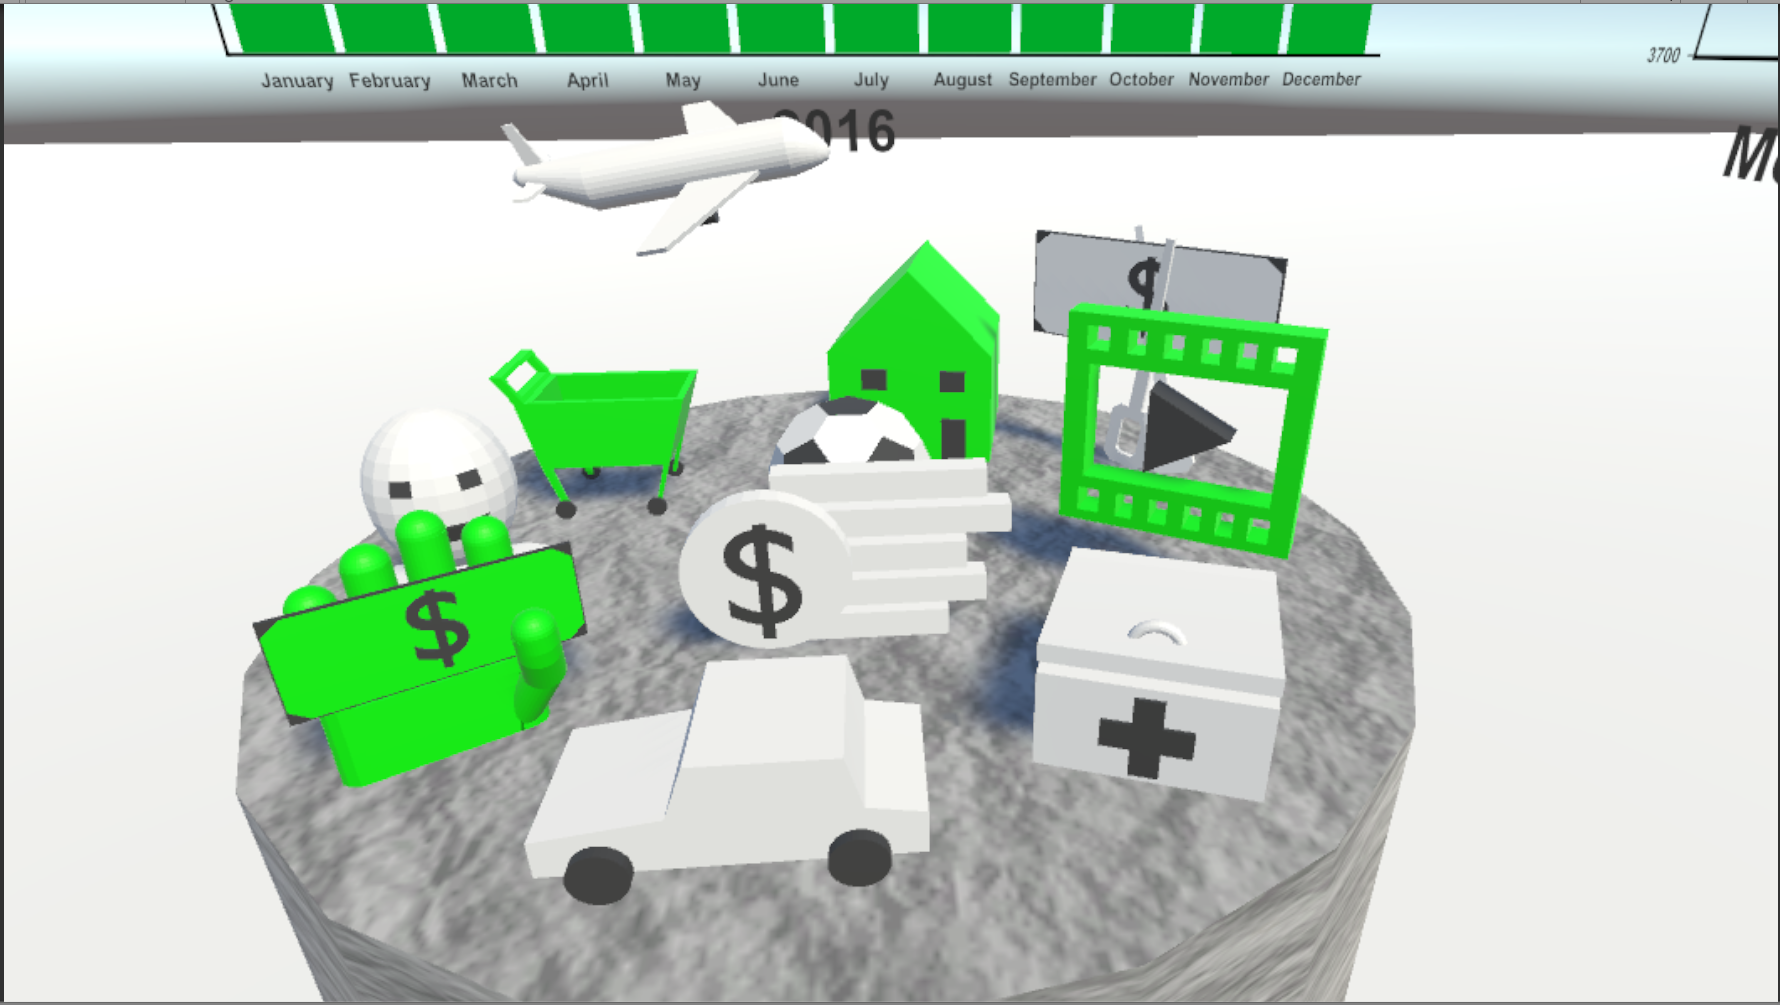
\includegraphics[width=2.35cm]{03_Figures/08_Development/View4_CategoriesFiltering.png}
		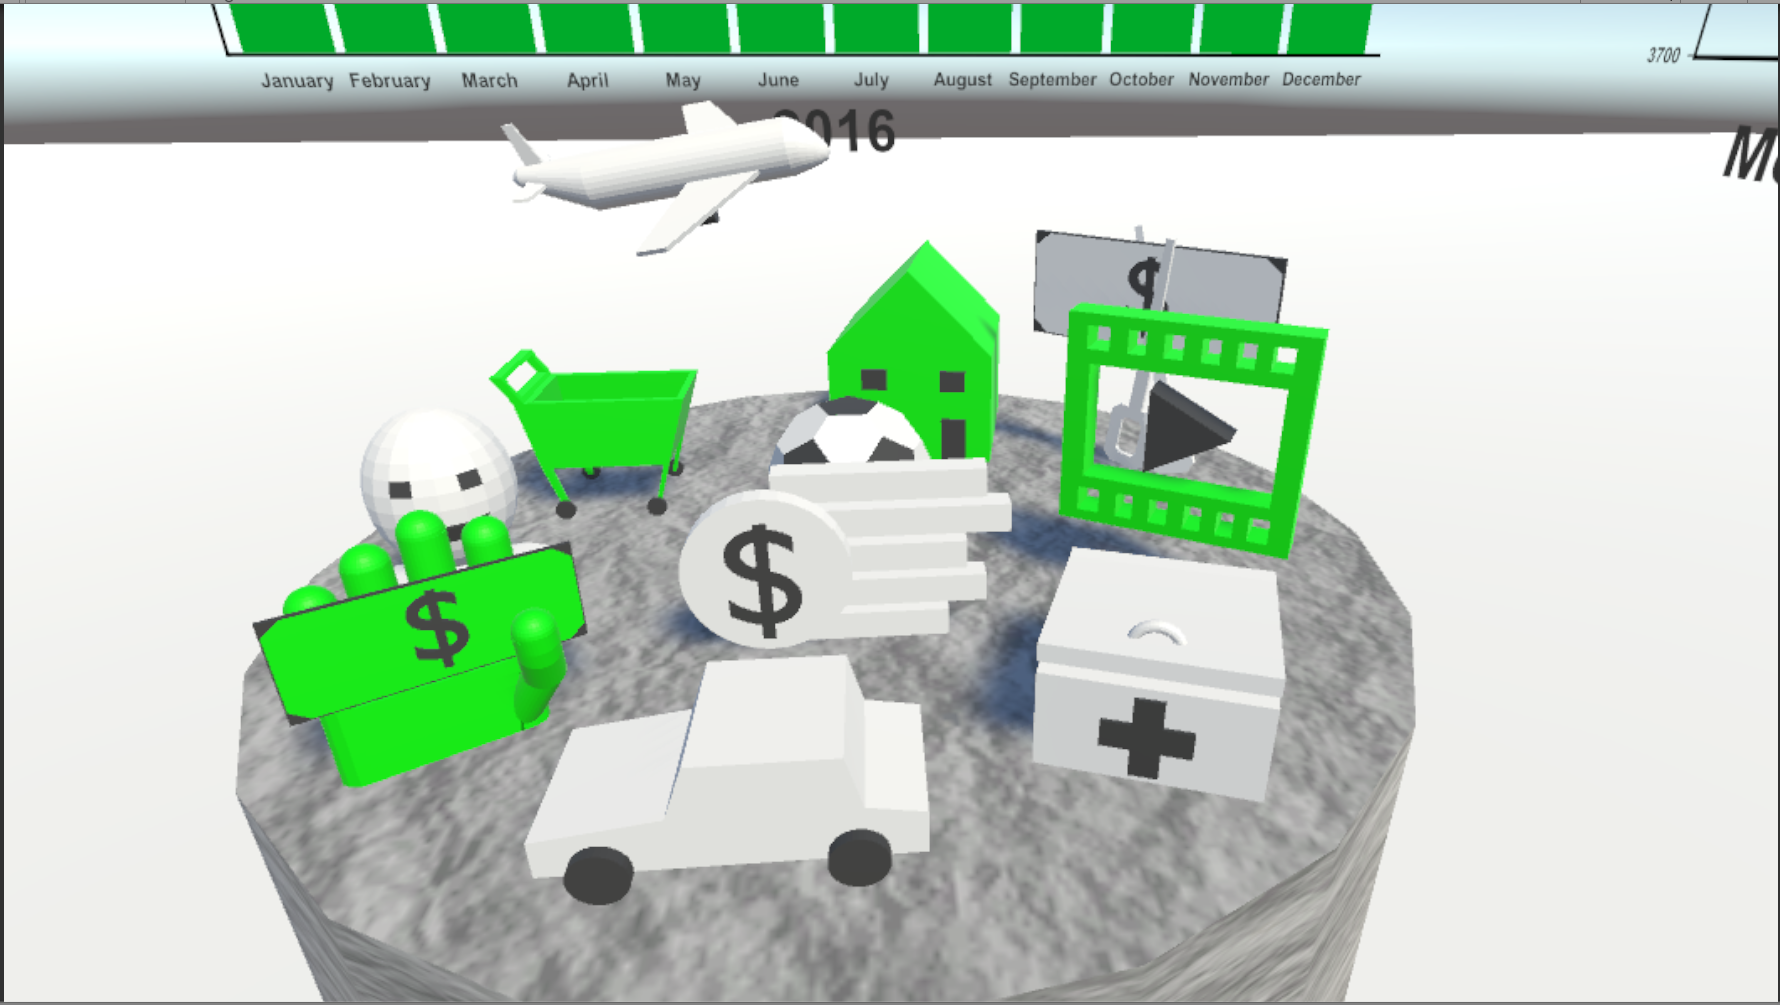
\includegraphics[width=2.35cm]{03_Figures/08_Development/View4_CategoriesFiltering.png}
		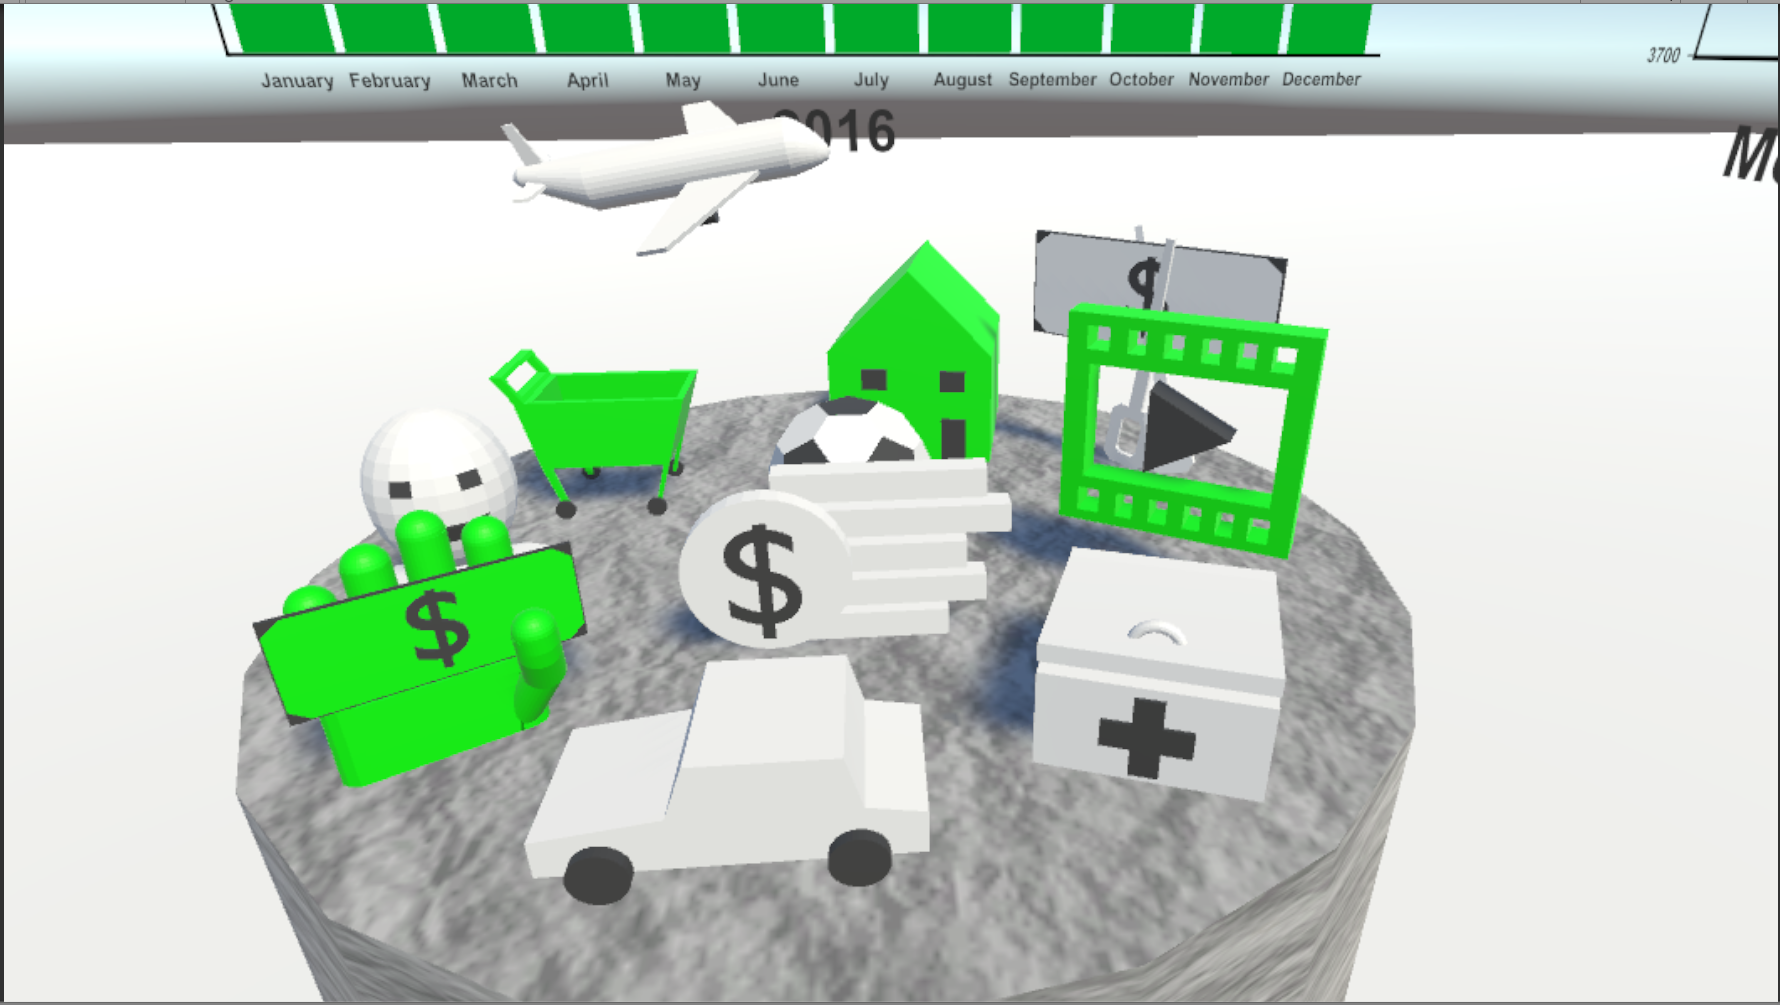
\includegraphics[width=2.35cm]{03_Figures/08_Development/View4_CategoriesFiltering.png}
		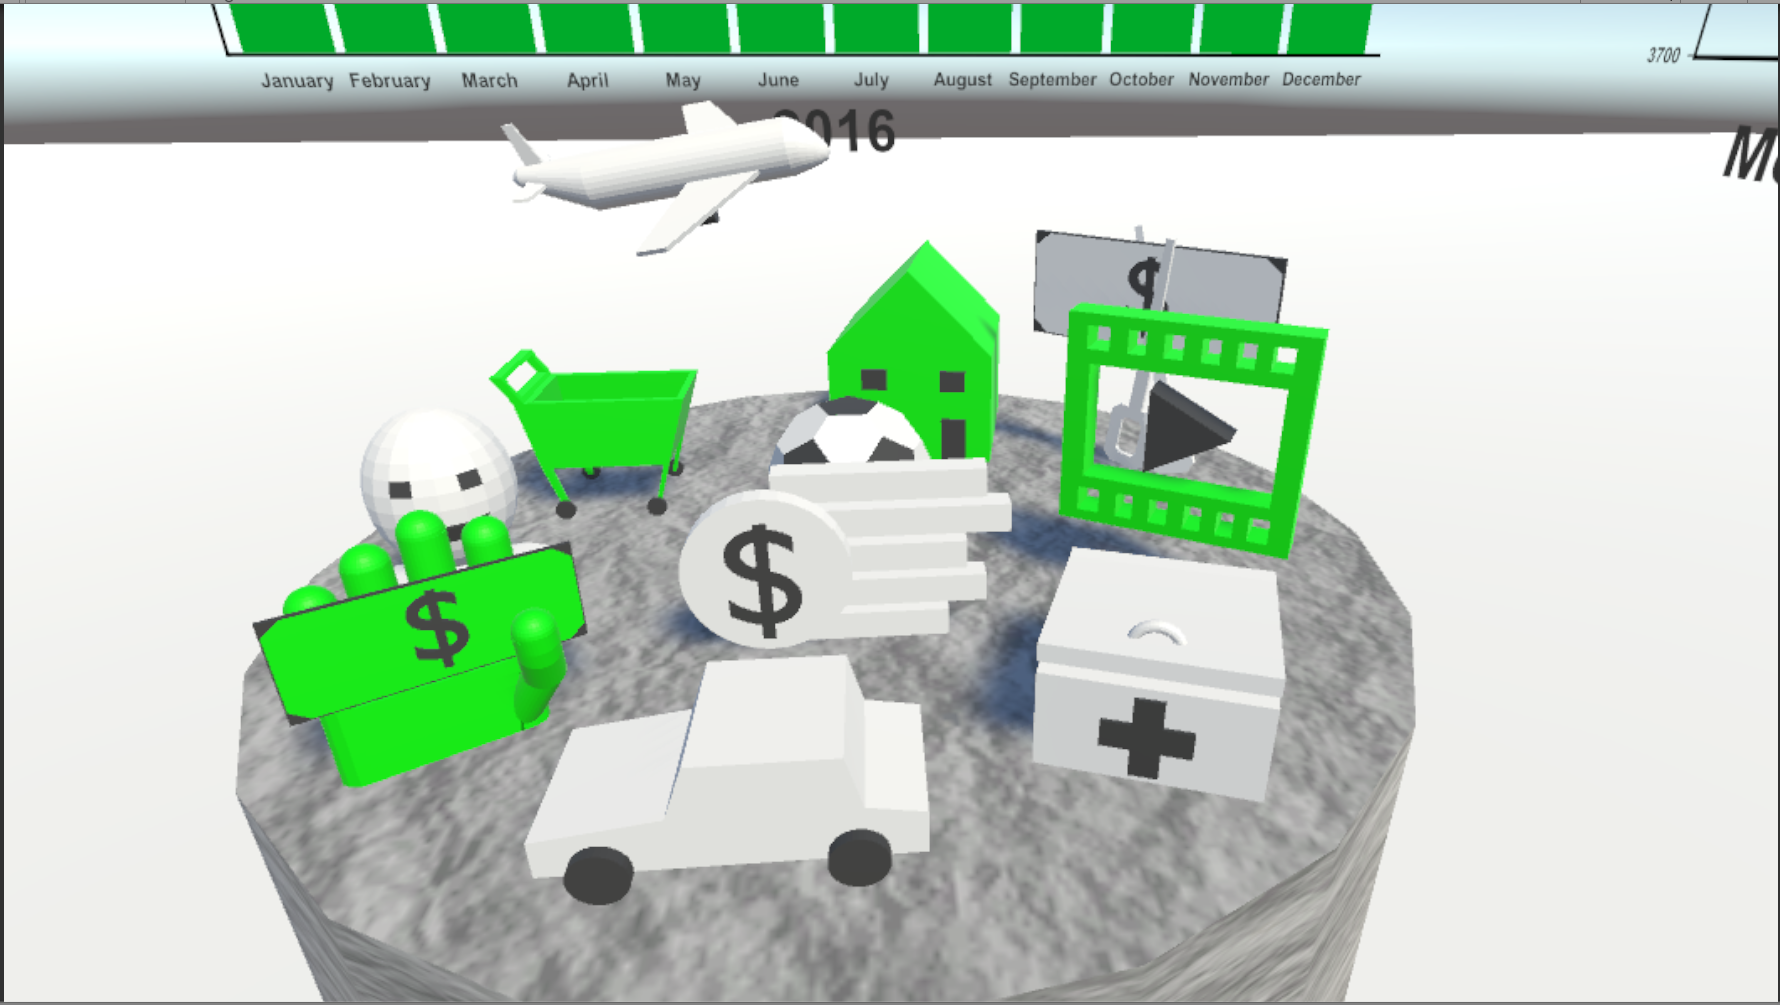
\includegraphics[width=2.35cm]{03_Figures/08_Development/View4_CategoriesFiltering.png}
		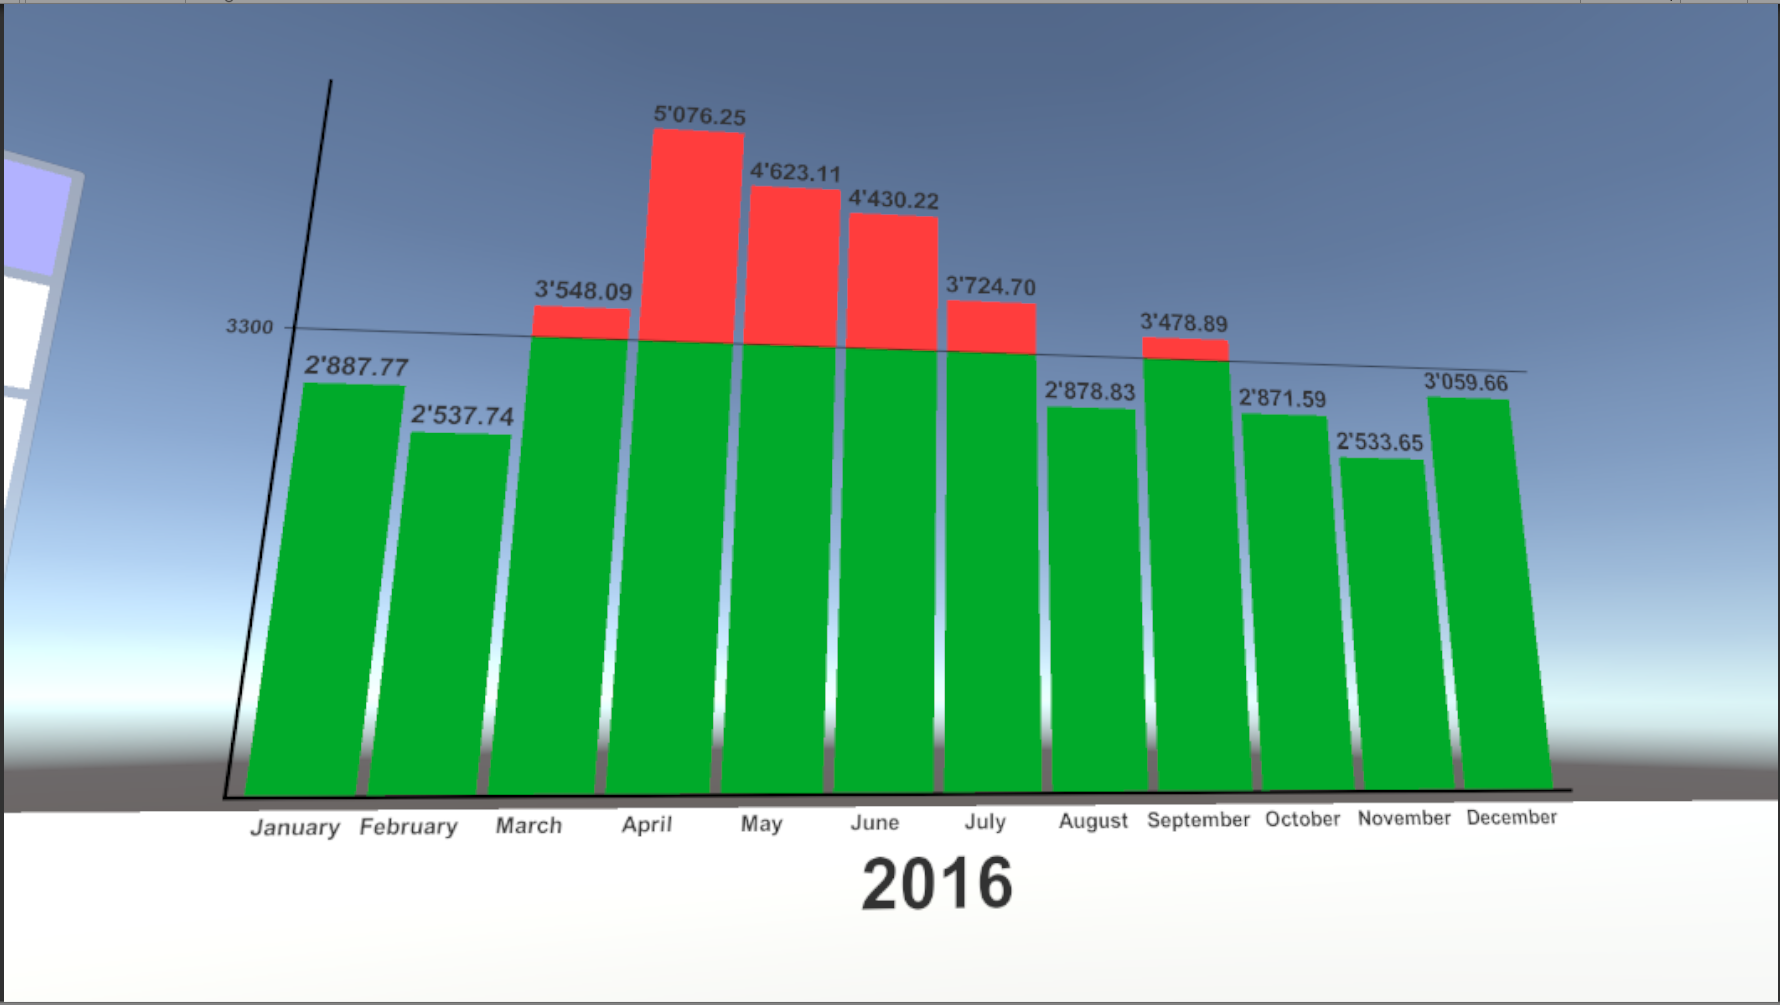
\includegraphics[width=2.35cm]{03_Figures/08_Development/View1_YearOverview.png}
		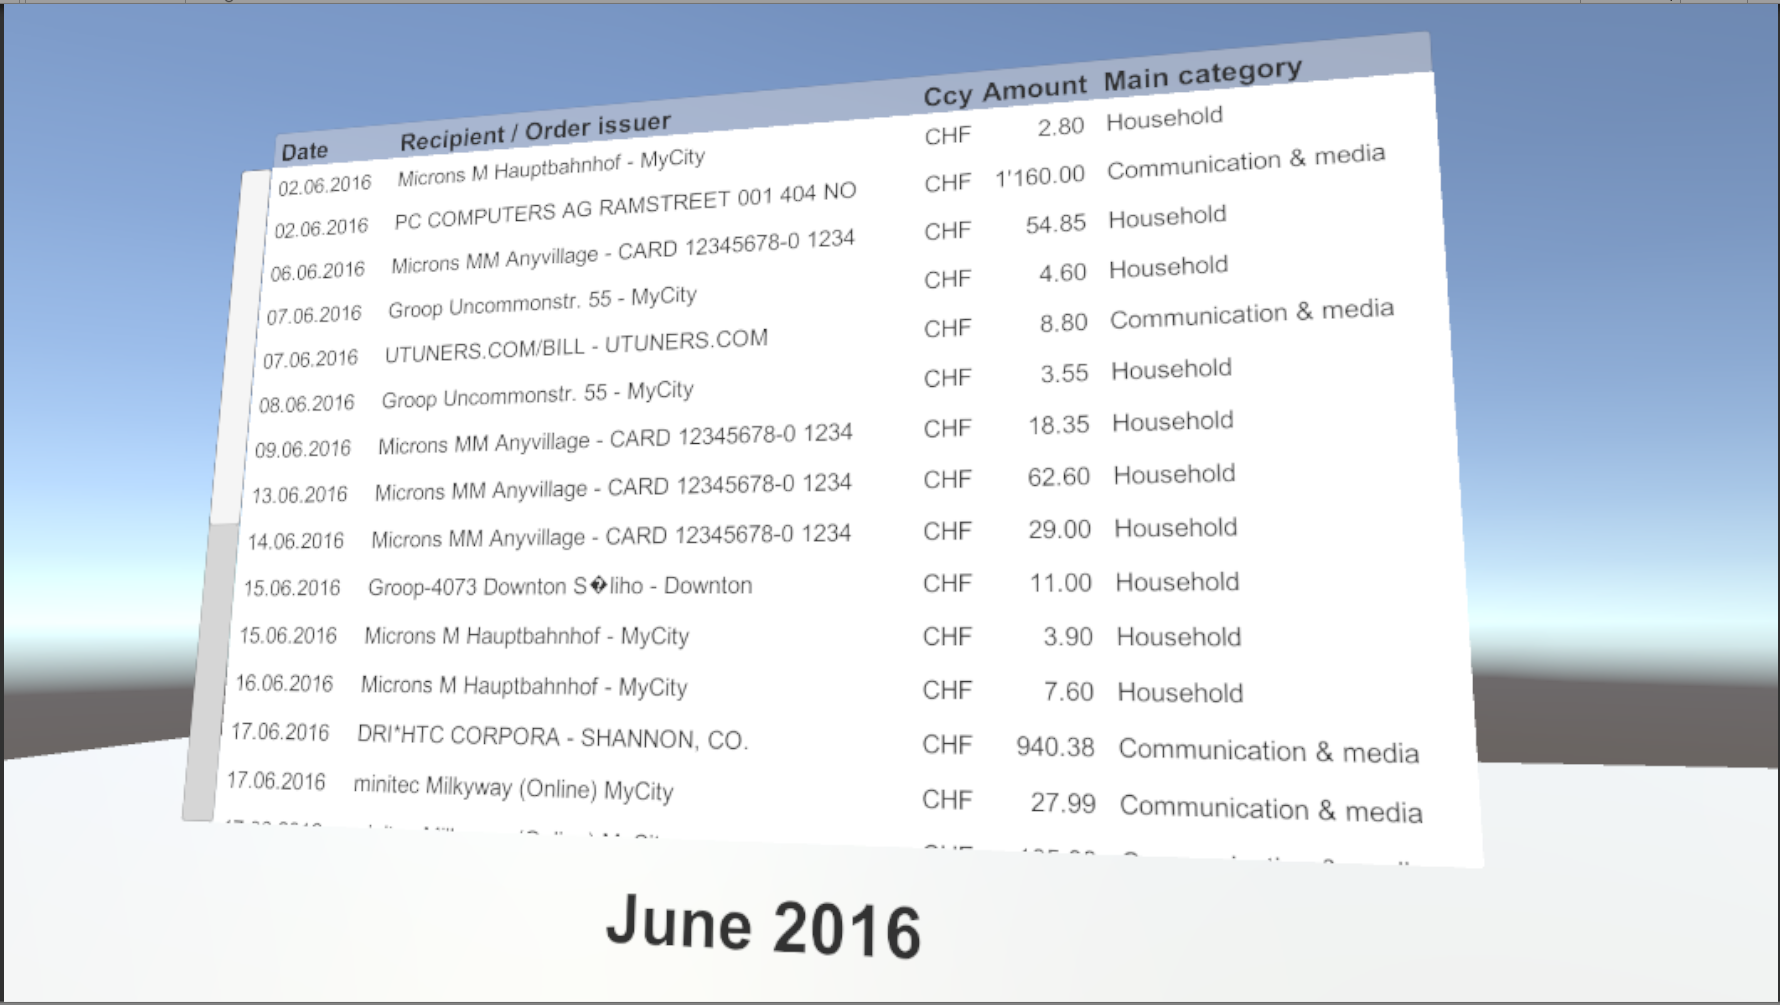
\includegraphics[width=2.35cm]{03_Figures/08_Development/View5_FinTransactionsOverview.png}
		\caption{Visualised flow of views in prototype for Scenario 4}
		\label{fig:scenariofourprototype}
	\end{center}
\end{figure}

\textbf{Evaluation:} The most interaction steps are spent on activating all relevant categories. Once the current month has been selected in the Year Overview, the Month Overview shows a cumulative chart with all expenses that can give an indication if and by when the threshold line might be reached if not already exceeded. For more details, the Transactions Overview table can be consulted on the right side to see what transaction had already been executed on the account. The exclusivity is only medium since the filtering does not go down to the sub-categories as potentially not the whole main category is relevant for this analysis. For the comprehensibility, again some interpretation is required in order to understand how much budget is left until the end of the month.
\begin{itemize}[noitemsep,nolistsep]
	\item Min. number of steps: \textbf{5 - 6}
	\item Exclusivity: \textbf{Medium}
	\item Comprehensibility: \textbf{Medium}
\end{itemize}


%-----------------------------------
%	SUBSUBSECTION 1
%-----------------------------------

\subsubsection{Conclusion}

tbd Table \ref{tbl:scenariofourcomparison}

\begin{table}[t]
	\begin{center}
		\begin{tabular}{ | p{3.5cm} | p{3cm} | p{3cm} | p{3cm} | } 
			\hline
			\textbf{Metric} & \textbf{E-banking} & \textbf{Prototype} & \textbf{Verdict} \\
			\hline
			Min. no. of steps: &  & 5 - 6 &  \\
			\hline
			Exclusivity: &  & Medium &  \\
			\hline
			Comprehensibility: &  & Medium &  \\
			\hline
		\end{tabular}
		\caption{Scenario 4: Comparison of prototype and e-banking}
		\label{tbl:scenariofourcomparison}
	\end{center}
\end{table}


%----------------------------------------------------------------------------------------
%	SECTION 2
%----------------------------------------------------------------------------------------

\section{Descriptive: Informed Arguments}

tbd
what is missing is guidance for how to perform the evaluation
TODO: Also check \cite{Peffers2012} for their definition of evaluation of a prototype


%-----------------------------------
%	SUBSECTION 1
%-----------------------------------
\subsection{tbd}

tbd




%-----------------------------------
%	SUBSECTION 2
%-----------------------------------

\subsection{tbd}

tbd




%----------------------------------------------------------------------------------------
%	SECTION 3
%----------------------------------------------------------------------------------------

\section{Conclusion}

tbd





